% ------------------------------------------------------------------------------
% TYPO3 Version 10 LTS - What's New (English Version)
%
% @author	Michael Schams <schams.net>
% @license	Creative Commons BY-NC-SA 3.0
% @link		https://typo3.org/help/documentation/whats-new/
% @language	English
% ------------------------------------------------------------------------------

\section{Systeemwijzigingen}
\begin{frame}[fragile]
	\frametitle{Systeemwijzigingen}

	\begin{center}\huge{\color{typo3darkgrey}\textbf{Systeemwijzigingen}}\end{center}
	\begin{center}\large{\textit{Verbeteringen en nieuwe functies voor integrators en ontwikkelaars}}\end{center}

\end{frame}

% ------------------------------------------------------------------------------
% Feature | 78432 | Add log message for Switch User action

\begin{frame}[fragile]
	\frametitle{Systeemwijzigingen}
	\framesubtitle{Gebruikerswissel in Backend}

	\begin{itemize}
		\item In de log is terug te vinden als een admin gebruiker wisselt naar een andere backend-gebruiker:
	\end{itemize}

	\begin{figure}
		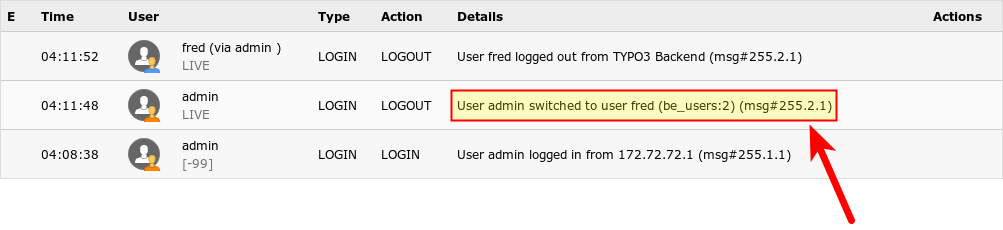
\includegraphics[width=0.90\linewidth]{InDepthChanges/78432-SwitchUserActionLogMessage.png}
	\end{figure}

\end{frame}

% ------------------------------------------------------------------------------
% Feature | 83734 | Add support for current page in configcache
% Breaking | 88564 | PageTSconfig setting TSFE.constants removed
% Breaking | 88657 | Popup configuration in FormEngine dropped

\begin{frame}[fragile]
	\frametitle{Systeemwijzigingen}
	\framesubtitle{Wijzigingen in TypoScript}

	\begin{itemize}
		\item TypoScript eigenschap \texttt{config.cache} ondersteunt het sleutelwoord
			"\texttt{current}" om te refereren aan de huidige pagina. Voorbeeld:\newline
			\smaller\texttt{config.cache.all = fe\_users:current}\normalsize

		\item De optie \texttt{TSFE.constants} in Page/User TSconfig is verwijderd.

			\begin{itemize}\smaller
				\item[\ding{228}] Gebruik TypoScript voorwaarden  in setup/constants en gebruik correcte configuratie in bestand \texttt{ext\_localconf.php}.
			\end{itemize}

		\item De volgende twee opties om de maat van een popup-venster in te stellen zijn verwijderd:

			\begin{itemize}
				\item \texttt{options.popupWindowSize}
				\item \texttt{options.rte.popupWindowSize}
			\end{itemize}

	\end{itemize}

\end{frame}

% ------------------------------------------------------------------------------
% Breaking | 88640 | Database field sys_template.nextLevel and TypoScript sublevel inheritance removed
% Task | 88755 | Remove POST option from typolink.addQueryString

\begin{frame}[fragile]
	\frametitle{Systeemwijzigingen}
	\framesubtitle{Wijzigingen in TypoScript}

	\begin{itemize}
		\item Het database-veld \texttt{nextLevel} van de database-tabel
			\texttt{sys\_template} zijn verwijderd.

			\begin{itemize}\smaller
				\item[\ding{228}] Vervang het record (het UID is opgeslagen in het veld \texttt{nextLevel}) met een voorwaarden om TypoScript toe te voegen voor onderliggende pagina's. Bijvoorbeeld: \texttt{[tree.level > 1]}
			\end{itemize}\normalsize

		\item De volgende waarden zijn \textbf{niet meer toegestaan}:

			\begin{itemize}\smaller
				\item \texttt{typolink.addQueryString.method = POST}
				\item \texttt{typolink.addQueryString.method = GET,POST}
				\item \texttt{typolink.addQueryString.method = POST,GET}
			\end{itemize}\normalsize

			\begin{itemize}\smaller
				\item[\ding{228}] Wijzig de waarden in TypoScript, Fluid en PHP naar \texttt{GET}.
			\end{itemize}\normalsize

	\end{itemize}

\end{frame}

% ------------------------------------------------------------------------------
% 87499 | Drop extensions "taskcenter" and "sys_action" from core

\begin{frame}[fragile]
	\frametitle{Systeemwijzigingen}
	\framesubtitle{Taakcentrum en \texttt{EXT:sys\_action}}

	\begin{itemize}

		\item De systeemextensies \texttt{EXT:taskcenter} en \texttt{EXT:sys\_action}
			zijn uit de core verwijderd.

		\item Ze zijn nu beschikbaar als aparte extensies in
			\href{https://extensions.typo3.org/}{TER}
			en op
			\href{https://github.com/FriendsOfTYPO3}{GitHub}.

		\item Het dashboard vervangt het taakcentrum en \texttt{EXT:sys\_action}.

	\end{itemize}

\end{frame}

% ------------------------------------------------------------------------------
% Feature | 89227 | Ask for email address while installing TYPO3

\begin{frame}[fragile]
	\frametitle{Systeemwijzigingen}
	\framesubtitle{E-mailadres beheerder}

	\begin{columns}[T]
		\begin{column}{.04\textwidth}
		\end{column}
		\begin{column}{.38\textwidth}

			Een e-mailadres kan nu ingevuld worden tijdens het installatieproces.
			Dit adres wordt gebruikt voor de backendgebruiker van de eerste beheerder.

			\vspace{0.2cm}

			Dezelfde optie is aanwezig in de Onderhoudsmodule van de Install Tool
			\textbf{Beheerder aanmaken}.

		\end{column}
		\begin{column}{.58\textwidth}
			\vspace{-0.3cm}
			\begin{figure}
				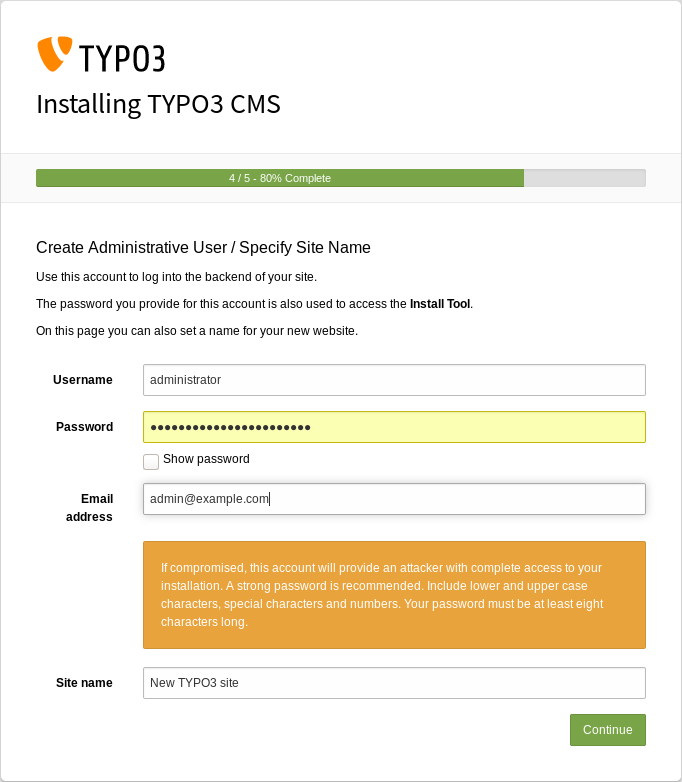
\includegraphics[width=0.70\linewidth]{InDepthChanges/89227-EmailAddressDuringInstallation.png}
			\end{figure}
		\end{column}
	\end{columns}

\end{frame}

% ------------------------------------------------------------------------------
% Breaking | 87583 | Remove obsolete APC Cache Backend implementation
% Breaking | 87558 | Consolidate extbase caches

\begin{frame}[fragile]
	\frametitle{Systeemwijzigingen}
	\framesubtitle{Caches}

	% decrease font size for code listing
	\lstset{basicstyle=\tiny\ttfamily}

	\begin{itemize}
		\item Het caching raamwerk ondersteunt de \texttt{ApcBackend} niet meer

			\begin{itemize}\smaller
				\item[\ding{228}] Gebruik \textbf{APCu} in plaats daarvan - let op de "u".
			\end{itemize}
\begin{lstlisting}
OUD:
$GLOBALS['TYPO3_CONF_VARS']['SYS']['caching']['cacheConfigurations']['rootline']['backend'] =
\TYPO3\CMS\Core\Cache\Backend\ApcBackend::class;

NIEUW:
$GLOBALS['TYPO3_CONF_VARS']['SYS']['caching']['cacheConfigurations']['rootline']['backend'] =
\TYPO3\CMS\Core\Cache\Backend\ApcuBackend::class;
\end{lstlisting}

		\item Extbase caches \texttt{extbase\_reflection} en \texttt{extbase\_datamapfactory\_datamap}
			zijn samengevoegd naar een cache met de naam "\texttt{extbase}".

	\end{itemize}

\end{frame}

% ------------------------------------------------------------------------------
% Feature | 89229 | Cache Preset for Settings in Maintenance Area

\begin{frame}[fragile]
	\frametitle{Systeemwijzigingen}
	\framesubtitle{Soort cacheopslag}

	\begin{itemize}

		\item TYPO3 biedt een flexibel cachesysteem met een standaardconfiguratie
			die perfect is voor de meeste gevallen.
		\item Het type opslage kan nu geconfigureerd worden om de caches af te regelen en
			de prestaties te verbeteren, afhankelijk van de eigen omgeving.

		\begin{itemize}
			\item Kies de \textbf{database}-opslag voor een standaardomgeving
				of als er een netwerkbestandssysteem (NFS) bijvoorbeeld gebruikt wordt.
			\item Kies het \textbf{bestandssysteem} als een gedistribueerde database
				bijvoorbeeld gebruikt wordt.
			\item Kies \textbf{aangepaste cache-instellingen} om het opslagtype
				voor elke cache apart te configureren.
		\end{itemize}

		\item Voor meer complexe installaties zouden geheugengebaseerde caches zoals
			\href{https://redis.io/}{Redis}
			of
			\href{https://memcached.org/}{Memcached}
			overwogen moeten worden.

	\end{itemize}

\end{frame}

% ------------------------------------------------------------------------------
% Feature | 89229 | Cache Preset for Settings in Maintenance Area

\begin{frame}[fragile]
	\frametitle{Systeemwijzigingen}
	\framesubtitle{Soort cacheopslag}

	Adminwerkset \ding{223}\hspace{0.1cm}Instellingen \ding{223}\hspace{0.1cm}Configuratievoorstellingen \ding{223}\hspace{0.1cm}Cache-instellingen:

	\begin{figure}
		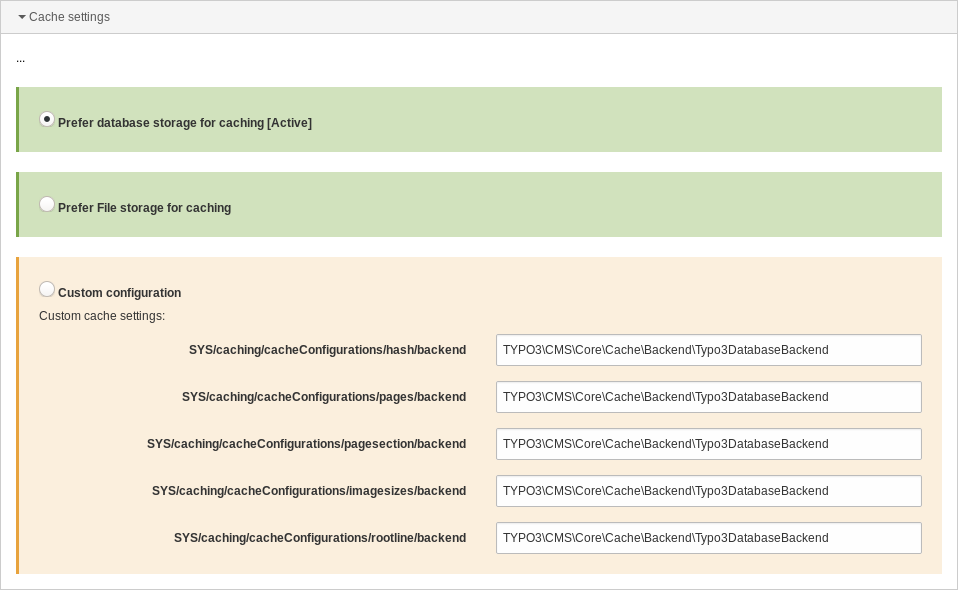
\includegraphics[width=0.70\linewidth]{InDepthChanges/89229a-CachePresetForSettingsInMaintenanceArea.png}
	\end{figure}

\end{frame}

% ------------------------------------------------------------------------------
% Feature | 89054 | Provide core cache frontends via dependency injection

\begin{frame}[fragile]
	\frametitle{Systeemwijzigingen}
	\framesubtitle{Afhankelijkheidsinjectie cache}

	% decrease font size for code listing
	\lstset{basicstyle=\tiny\ttfamily}

	\begin{itemize}
		\item Extensieontwikkelaars wordt aangeraden om caches direct te injecteren i.p.v. de CacheManager
			te gebruiker.
		\item Dit vergt enkele simpele wijzigingen zoals hieronder.

		\item \textbf{Previously:}
\begin{lstlisting}
class MyClass
{
  /**
   * @var TYPO3\CMS\Core\Cache\Frontend\FrontendInterface
   */
  private $cache;

  public function __construct()
  {
      $cacheManager = GeneralUtility::makeInstance(CacheManager::class);
      $this->cache = $cacheManager->getCache('my_cache');
  }
}
\end{lstlisting}

	\end{itemize}

\end{frame}

% ------------------------------------------------------------------------------
% Feature | 89054 | Provide core cache frontends via dependency injection

\begin{frame}[fragile]
	\frametitle{Systeemwijzigingen}
	\framesubtitle{Afhankelijkheidsinjectie cache}

	% decrease font size for code listing
	\lstset{basicstyle=\tiny\ttfamily}

	\begin{itemize}
		\item Sinds \textbf{TYPO3 v10.1}, zou de klasse er zo uit moeten zien:
\begin{lstlisting}
class MyClass
{
  /**
   * @var TYPO3\CMS\Core\Cache\Frontend\FrontendInterface
   */
  private $cache;

  public function __construct(FrontendInterface $cache)
  {
    $this->cache = $cache;
  }
}
\end{lstlisting}

	\end{itemize}

\end{frame}

% ------------------------------------------------------------------------------
% Feature | 89054 | Provide core cache frontends via dependency injection

\begin{frame}[fragile]
	\frametitle{Systeemwijzigingen}
	\framesubtitle{Afhankelijkheidsinjectie cache}

	% decrease font size for code listing
	\lstset{basicstyle=\tiny\ttfamily}

	\begin{itemize}
		\item ...en de volgende configuratie van de container-service is nodig:
\begin{lstlisting}
services:
  cache.my_cache:
    class: TYPO3\CMS\Core\Cache\Frontend\FrontendInterface
    factory: ['@TYPO3\CMS\Core\Cache\CacheManager', 'getCache']
    arguments: ['my_cache']

  MyClass:
    arguments:
      $cache: '@cache.my_cache'
\end{lstlisting}

	\end{itemize}

\end{frame}

% ------------------------------------------------------------------------------
% Deprecation | 88366 | Default caching framework cache names changed

\begin{frame}[fragile]
	\frametitle{Systeemwijzigingen}
	\framesubtitle{Caching Framework}

	% decrease font size for code listing
	\lstset{basicstyle=\tiny\ttfamily}

	\begin{itemize}
		\item De volgende caches zijn hernoemd:

			\begin{itemize}\smaller
				\item \texttt{cache\_core} \textrightarrow\hspace{0.1cm}\texttt{core}
				\item \texttt{cache\_hash} \textrightarrow\hspace{0.1cm}\texttt{hash}
				\item \texttt{cache\_pages} \textrightarrow\hspace{0.1cm}\texttt{pages}
				\item \texttt{cache\_pagesection} \textrightarrow\hspace{0.1cm}\texttt{pagesection}
				\item \texttt{cache\_runtime} \textrightarrow\hspace{0.1cm}\texttt{runtime}
				\item \texttt{cache\_rootline} \textrightarrow\hspace{0.1cm}\texttt{rootline}
				\item \texttt{cache\_imagesizes} \textrightarrow\hspace{0.1cm}\texttt{imagesizes}
			\end{itemize}\normalsize

		\item Nieuwe methode om de cache te benaderen:
\begin{lstlisting}
OUD:
$cacheManager->getCache('cache_core').

NIEUW:
$cacheManager->getCache('core')
\end{lstlisting}

		\item Het voorvoegsel \texttt{cf\_} is verwijderd uit de database tabellen.
	\end{itemize}

\end{frame}

% ------------------------------------------------------------------------------
% Feature | 89090 | Reports for conflicting redirects

\begin{frame}[fragile]
	\frametitle{Systeemwijzigingen}
	\framesubtitle{Conflicterende doorverwijzingen}

	\begin{itemize}
		\item Er is een nieuw Symfony commando om doorverwijzingen te detecteren
			die conflicteren met pagina-URL's.
		\item Voer het commando uit op de commandoregel:\newline
			\smaller
				(optionele parameter \texttt{-}\texttt{-site} beperkt de controle tot een specifieke site)
			\normalsize
	\end{itemize}

	\begin{figure}
		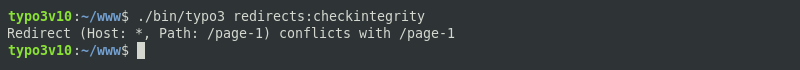
\includegraphics[width=0.90\linewidth]{InDepthChanges/89090a-ReportsForConflictingRedirects.png}
	\end{figure}

	\begin{itemize}
		\item Het commando is ook beschikbaar als een taakplannertaak:
	\end{itemize}

	\begin{figure}
		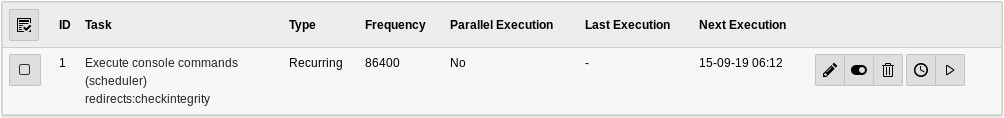
\includegraphics[width=0.90\linewidth]{InDepthChanges/89090b-ReportsForConflictingRedirects.png}
	\end{figure}

\end{frame}

% ------------------------------------------------------------------------------
% Feature | 89090 | Reports for conflicting redirects

\begin{frame}[fragile]
	\frametitle{Systeemwijzigingen}
	\framesubtitle{Conflicting Redirects}

	\begin{itemize}
		\item Een lijst met gevonden conflicterende doorverwijzingen is ook te vinden in de module Rapportage:
	\end{itemize}

	\begin{figure}
		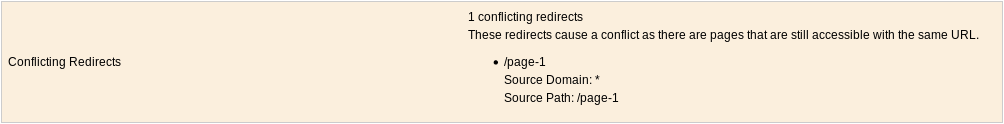
\includegraphics[width=0.90\linewidth]{InDepthChanges/89090c-ReportsForConflictingRedirects.png}
	\end{figure}

	\begin{itemize}
		\item
			\small\textbf{Let op:}
				Het commando moet weer uitgevoerd worden om de lijst te "herbouwen".
				Het oplossen van het probleem (bijv. de doorverwijzing verwijderen) maakt de lijst niet leeg.
			\normalsize
	\end{itemize}

\end{frame}

% ------------------------------------------------------------------------------
% Feature | 89010 | Introduce Site Configuration for Distribution Packages

\begin{frame}[fragile]
	\frametitle{Systeemwijzigingen}
	\framesubtitle{Distributiepakketten}

	% decrease font size for code listing
	\lstset{basicstyle=\tiny\ttfamily}

	\begin{itemize}
		\item Distributies kunnen nu een siteconfguratie bestand(en) bevatten.

		\item Maak een map/bestand in het distributiepakket aan als volgt:\newline
			\texttt{Initialisation/Site/<siteIdentifier>/config.yaml}

		\item Net zoals met bestanden die verplaatst worden naar \texttt{fileadmin/},\newline
			wordt siteconfiguratie verplaatst naar de map \texttt{config/}.

		\item Als de doelmap al bestaat wordt de bestaande configuratie niet gewijzigd.
	\end{itemize}

\end{frame}

% ------------------------------------------------------------------------------
% Feature | 88318 | Display Application Context in CLI

\begin{frame}[fragile]
	\frametitle{Systeemwijzigingen}
	\framesubtitle{Applicatiecontext in CLI}

	\begin{itemize}
		\item De huidige applicatiecontext wordt nu getoond naast het
			TYPO3 versienummer op de opdrachtregel:
	\end{itemize}

	\begin{figure}
		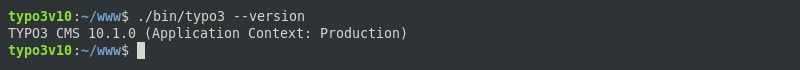
\includegraphics[width=0.90\linewidth]{InDepthChanges/88318-DisplayApplicationContextInCli.png}
	\end{figure}

\end{frame}

% ------------------------------------------------------------------------------
% Feature | 87525 | Add api=1 option in VimeoRenderer

\begin{frame}[fragile]
	\frametitle{Systeemwijzigingen}
	\framesubtitle{Vimeo Video Weergave}

	% decrease font size for code listing
	\lstset{basicstyle=\smaller\ttfamily}

	\begin{itemize}
		\item De parameter \texttt{api=1} in Vimeo video URL's maakt API-interactie met de videospeler
			(bijv. extra knoppen om de video te bedienen) mogelijk.
	\item Integrators kunnen deze parameter op twee manieren instellen.

		\begin{itemize}
			\item Met TypoScript:
\begin{lstlisting}
lib.contentElement.settings.media.additionalConfig.api = 1
\end{lstlisting}

			\item In Fluid met de Media-ViewHelper:
\begin{lstlisting}
<f:media
  file="{file}"
  alt="{file.properties.alternative}"
  title="{file.properties.title}"
  additionalConfig="{api: 1}"
/>
\end{lstlisting}

		\end{itemize}
	\end{itemize}

\end{frame}

% ------------------------------------------------------------------------------
% Feature | 86670 | Make default action in DragUploader adjustable

\begin{frame}[fragile]
	\frametitle{Systeemwijzigingen}
	\framesubtitle{Bestandsuploads}

	% decrease font size for code listing
	\lstset{basicstyle=\smaller\ttfamily}

	\begin{itemize}
		\item De standaardactie bij het uploaden van bestanden via verslepen in de bestandslijst module kan nu ingesteld worden.
		\item User TSConfig:
\begin{lstlisting}
# Standaard vervangen:
options.file_list.uploader.defaultAction = replace

# Standaard hernoemen:
options.file_list.uploader.defaultAction = rename

# Standaard annuleren:
options.file_list.uploader.defaultAction = cancel
\end{lstlisting}

	\end{itemize}

\end{frame}

% ------------------------------------------------------------------------------
% Feature | 84250 | Separately enable / disable "Add media by URL" and "Select & upload files"

\begin{frame}[fragile]
	\frametitle{Systeemwijzigingen}
	\framesubtitle{Media-elementknoppen}

	% decrease font size for code listing
	\lstset{basicstyle=\tiny\ttfamily}

	\begin{itemize}
		\item Knoppen \textbf{"Media toevoegen op URL"} en \textbf{"Kiezen \& bestanden uploaden"}
			kunnen nu onafhankelijk van elkaar in-/uitgeschakeld worden.
	\end{itemize}

	\begin{figure}
		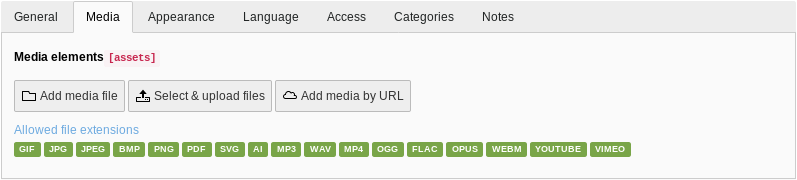
\includegraphics[width=0.75\linewidth]{InDepthChanges/84250-EnableDisableMediaButtons.png}
	\end{figure}

	\begin{itemize}
		\item Dit voorbeeld verbergt beide knoppen:
\begin{lstlisting}
$GLOBALS['TCA']['pages']['columns']['media']['config']['appearance'] = [
  'fileUploadAllowed' => false,
  'fileByUrlAllowed' => false,
];
\end{lstlisting}

	\end{itemize}

\end{frame}

% ------------------------------------------------------------------------------
% Feature | 88441 | Show configuration of USER_INT objects in adminpanel

\begin{frame}[fragile]
	\frametitle{Systeemwijzigingen}
	\framesubtitle{Admin-paneel}

	\begin{itemize}
		\item Het admin-paneel heeft een nieuw onderdeel \textbf{USER\_INT} in de "Info" module.
	\end{itemize}

	\begin{figure}
		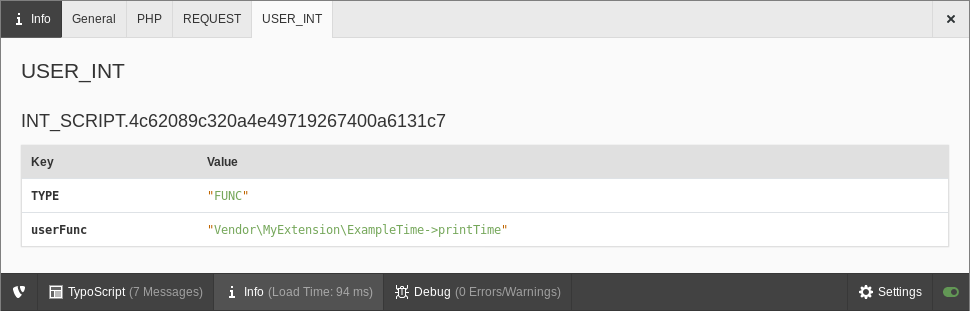
\includegraphics[width=0.90\linewidth]{InDepthChanges/88441-ShowUserIntObjectsInAdminPanel.png}
	\end{figure}

\end{frame}

% ------------------------------------------------------------------------------
% Feature | 89142 | Create site configuration if page is created on root level

\begin{frame}[fragile]
	\frametitle{Systeemwijzigingen}
	\framesubtitle{Site-configuratie}

	\begin{itemize}
		\item Als een nieuwe pagina op het rootniveau wordt aangemaakt wordt een
			standaard siteconfiguratie automatisch gegenereerd.
		\item Dit maakt dat een basis TYPO3-site snel opgezet kan worden.
		\item De siteconfiguratiefuncties:

		\begin{itemize}
			\item een voorgedefinieerde identifier (bijv. \texttt{site-42-a1d0c6e83f})
			\item een beginpunt (bijv. \texttt{https://example.com/site-42})
			\item een standaardtaal (bijv. \texttt{English})
		\end{itemize}

	\end{itemize}

\end{frame}

% ------------------------------------------------------------------------------
% Feature | 85592 | Add site title configuration to sites module

\begin{frame}[fragile]
	\frametitle{Systeemwijzigingen}
	\framesubtitle{Site-configuratie}

	\begin{itemize}

		\item De titel van de site kan nu geconfigureerd worden in
			\textbf{Site Configuratie} $\rightarrow$ \textbf{Sites}.
		\item Dit geeft integrators de mogelijkheid een site-titel per taal in te stellen.
		\item Het veld in de sjabloonrecord is overbodig en is als \textbf{verouderd} gemarkeerd.
		\item Het veld \texttt{sys\_template.sitetitle} (database en TCA) zal worden verwijderd in TYPO3 v11.
		\item De titel van de site wordt gebruikt voor de paginatitel en ook voor toekomstige
			\texttt{schema.org} integraties.
	\end{itemize}

\end{frame}

% ------------------------------------------------------------------------------
% Feature | 89398 | Support for environment variables in imports in site configurations

\begin{frame}[fragile]
	\frametitle{Systeemwijzigingen}
	\framesubtitle{Site-configuratie}

	% decrease font size for code listing
	\lstset{basicstyle=\tiny\ttfamily}

	\begin{itemize}

		\item Het is nu mogelijk om omgevingsvariabelen te gebruiken in imports van siteconfiguratie YAML bestanden:
\begin{lstlisting}
imports:
  -
    resource: 'Env_%env("foo")%.yaml'
\end{lstlisting}

	\end{itemize}

\end{frame}

% ------------------------------------------------------------------------------
% Feature | 88102 | Frontend Login Form Via Fluid And Extbase

\begin{frame}[fragile]
	\frametitle{Systeemwijzigingen}
	\framesubtitle{Aanmelding Frontend}

	\begin{itemize}

		\item TYPO3 v10.2 bevat nu een Extbase-versie van de functionaliteit voor het aanmelden in de frontend.
		\item Deze oplossing heeft een aantal voordelen:

			\begin{itemize}
				\item Eenvoudiger sjablonen aanpassen.
				\item Verstuur wachtwoord vergeten e-mails gebaseerd op HTML.
				\item Instellen en aanpassen van validators om wachtwoordrestricties te forceren.
			\end{itemize}

		\item De nieuwe Extbase plugin is standaard beschikbaar voor nieuwe installaties.
		\item Bestaande installaties blijven gebruik maken van de oude sjablonen.
		\item Integrators kunnen wisselen tussen de "oude" en de "nieuwe" plug-in met een functieschakelaar.

	\end{itemize}

\end{frame}

% ------------------------------------------------------------------------------
% Feature | 88110 | Felogin extbase password recovery

\begin{frame}[fragile]
	\frametitle{Systeemwijzigingen}
	\framesubtitle{Aanmelding Frontend}

	\begin{itemize}

		\item Aan de Extbase plug-in is een wachtwoord-vergeten-formulier toegevoegd.
		\item Gebruikers kunnen aangeven het wachtwoord opnieuw te willen instellen. Ze krijgen vervolgens een e-mail met een link naar het formulier.
		\item Standaard wachtwoordvalidatieregels:

			\begin{itemize}
				\item \texttt{NotEmptyValidator} - wachtwoorden mogen niet leeg zijn.
				\item \texttt{StringLengthValidator} - wachtwoorden moeten een minimale lengte hebben.
			\end{itemize}

	\end{itemize}

\end{frame}

% ------------------------------------------------------------------------------
% Feature | 88110 | Felogin extbase password recovery

\begin{frame}[fragile]
	\frametitle{Systeemwijzigingen}
	\framesubtitle{Aanmelding Frontend}

	% decrease font size for code listing
	\lstset{basicstyle=\tiny\ttfamily}

	\begin{itemize}
		\item De validatieregels kunnen worden aangepast.
		\item Bijvoorbeeld:
\begin{lstlisting}
plugin.tx_felogin_login {
  settings {
    passwordValidators {
      10 = TYPO3\CMS\Extbase\Validation\Validator\AlphanumericValidator
      20 {
        className = TYPO3\CMS\Extbase\Validation\Validator\StringLengthValidator
        options {
          minimum = 12
          maximum = 32
        }
      }
      30 = \Vendor\MyExtension\Validation\Validator\MyCustomPasswordPolicyValidator
    }
  }
}
\end{lstlisting}

	\end{itemize}

\end{frame}

% ------------------------------------------------------------------------------
% Feature | 89171 | Added possibility to have multiple sitemaps

\begin{frame}[fragile]
	\frametitle{Systeemwijzigingen}
	\framesubtitle{Meerdere sitemaps}

	% decrease font size for code listing
	\lstset{basicstyle=\tiny\ttfamily}

	\begin{itemize}

		\item Het is nu mogelijk om meerdere sitemaps te configureren.
		\item Voorbeeld:
\begin{lstlisting}
plugin.tx_seo {
  config {
    <sitemapType> {
      sitemaps {
        <unique key> {
          provider = TYPO3\CMS\Seo\XmlSitemap\RecordsXmlSitemapDataProvider
          config {
            ...
          }
        }
      }
    }
  }
}
\end{lstlisting}

	\end{itemize}

\end{frame}

% ------------------------------------------------------------------------------
% Feature | 86759 | Support nomodule attribute for JavaScript includes

\begin{frame}[fragile]
	\frametitle{Systeemwijzigingen}
	\framesubtitle{HTML5 attribuut \texttt{nomodule}}

	% decrease font size for code listing
	\lstset{basicstyle=\tiny\ttfamily}

	\begin{itemize}
		\item Het HTML5 attribuut \texttt{nomodule} wordt nu ondersteund bij het inladen van JavaScript-bestanden via TypoScript.
\begin{lstlisting}
page.includeJSFooter.file = path/to/classic-file.js
page.includeJSFooter.file.nomodule = 1
\end{lstlisting}

		\item Dit attribuut voorkomt dat het script wordt uitgevoerd wanneer de browser modulescripts ondersteunt.

		\item Lees meer over deze standaard in de
			\href{https://html.spec.whatwg.org/multipage/scripting.html#attr-script-nomodule}{specificatie}
			en over het concept van
			\href{https://hacks.mozilla.org/2015/08/es6-in-depth-modules/}{modules}.

	\end{itemize}

% <script type="module" src="path/to/file.js"></script>
% <script nomodule src="path/to/file/classic-file.js"></script>

\end{frame}

% ------------------------------------------------------------------------------
% Feature | 86918 | Add additional configuration for external link types in Linkvalidator

\begin{frame}[fragile]
	\frametitle{Systeemwijzigingen}
	\framesubtitle{Link Validator}

	% decrease font size for code listing
	\lstset{basicstyle=\tiny\ttfamily}

	\begin{itemize}
		\item De Link Validator ondersteunt nu extra configuratie voor externe links.
		\item Waarden voor \texttt{httpAgentUrl} en \texttt{httpAgentEmail} moeten worden opgegeven.
		\item De instellingen \texttt{headers}, \texttt{method} en \texttt{range} zijn geavanceerde instellingen.
\begin{lstlisting}
mod.linkvalidator {
  linktypesConfig {
    external {
      httpAgentName = ...
      httpAgentUrl = ...
      httpAgentEmail = ...
      headers {
      }
      method = HEAD
      range = 0-4048
    }
  }
}
\end{lstlisting}

	\end{itemize}

\end{frame}

% ------------------------------------------------------------------------------
% Feature | 84990 | Add event for checking external links in RTE

\begin{frame}[fragile]
	\frametitle{Systeemwijzigingen}
	\framesubtitle{Link Validator}

	\begin{itemize}
		\item De Link Validator markeert nu ook kapotte \textbf{externe} links in de RTE.
		\item Deze functie was alleen beschikbaar voor interne links.
		\item Het wordt aangeraden om de Link Validator in de Taakplanner uit te voeren om regelmatig te controleren op kapotte links.
	\end{itemize}

\end{frame}

% ------------------------------------------------------------------------------



% ------------------------------------------------------------------------------
% Important | 89992 | Use New TranslationServer
% Feature | 89526 | FeatureFlag: betaTranslationServer

\begin{frame}[fragile]
	\frametitle{Systeemwijzigingen}
	\framesubtitle{Localization Management Platform}

	\begin{itemize}
		\item De SaaS-oplossing "\href{https://crowdin.com/}{Crowdin}" wordt nu gebruikt als
			het platform voor het beheer van vertalingen voor TYPO3.
		\item We moedigen iedereen aan mee te doen en de vertalingen te verbeteren.
		\item Crowdin van gebruikt worden om de labels van de TYPO3 core te vertalen
			maar ook die van TYPO3 extensies.
		\item Lees meer hierover in
			\href{https://typo3.org/community/teams/typo3-development/initiatives/localization-with-crowdin/}{dit artikel}
			en in de
			\href{https://docs.typo3.org/m/typo3/reference-coreapi/master/en-us/ApiOverview/Internationalization/TranslationServer/Crowdin.html}{TYPO3 documentatie}.
	\end{itemize}

	\begin{figure}
		
\includegraphics[width=0.40\linewidth]{InDepthChanges/crowdin-logo.png}
	\end{figure}

\end{frame}

% ------------------------------------------------------------------------------
% Feature | 90266 | Fluid-based templated emails

\begin{frame}[fragile]
	\frametitle{Systeemwijzigingen}
	\framesubtitle{Fluid voor HTML e-mails}

	% decrease font size for code listing
	\lstset{basicstyle=\smaller\ttfamily}

	\begin{itemize}
		\item TYPO3 ondersteunt nu het versturen van HTML en tekst e-mails op basis van sjablonen.
		\item E-mails worden gebouwd met Fluid sjablonen.
		\item E-mailsjablonen kunnen aangepast worden door de paden naar de sjabloonbestanden te overschrijven:
\begin{lstlisting}
$GLOBALS['TYPO3_CONF_VARS']['MAIL']['templateRootPaths'][700] =
  'EXT:my_site_extension/Resources/Private/Templates/Email';

$GLOBALS['TYPO3_CONF_VARS']['MAIL']['layoutRootPaths'][700] =
  'EXT:my_site_extension/Resources/Private/Layouts';
\end{lstlisting}

	\end{itemize}

\end{frame}

% ------------------------------------------------------------------------------
% Feature | 90266 | Fluid-based templated emails

\begin{frame}[fragile]
	\frametitle{Systeemwijzigingen}
	\framesubtitle{Fluid voor HTML e-mails}

	\begin{itemize}
		\item E-mail gebaseerd op Fluid-sjablonen worden bijvoorbeeld bij de volgende componenten gebruikt:

			\begin{itemize}
				\item Install Tool test e-mail (zie voorbeeld op volgende dia).
				\item Werkruimtenotificaties bij stadiumwijziging.
				\item Notificaties bij het inloggen van backend-gebruikers.
			\end{itemize}

	\end{itemize}

\end{frame}

% ------------------------------------------------------------------------------
% Feature | 90266 | Fluid-based templated emails

\begin{frame}[fragile]
	\frametitle{Systeemwijzigingen}
	\framesubtitle{Fluid voor HTML e-mails}

	Test-e-mail verstuurd door de Install Tool:

	\begin{figure}
		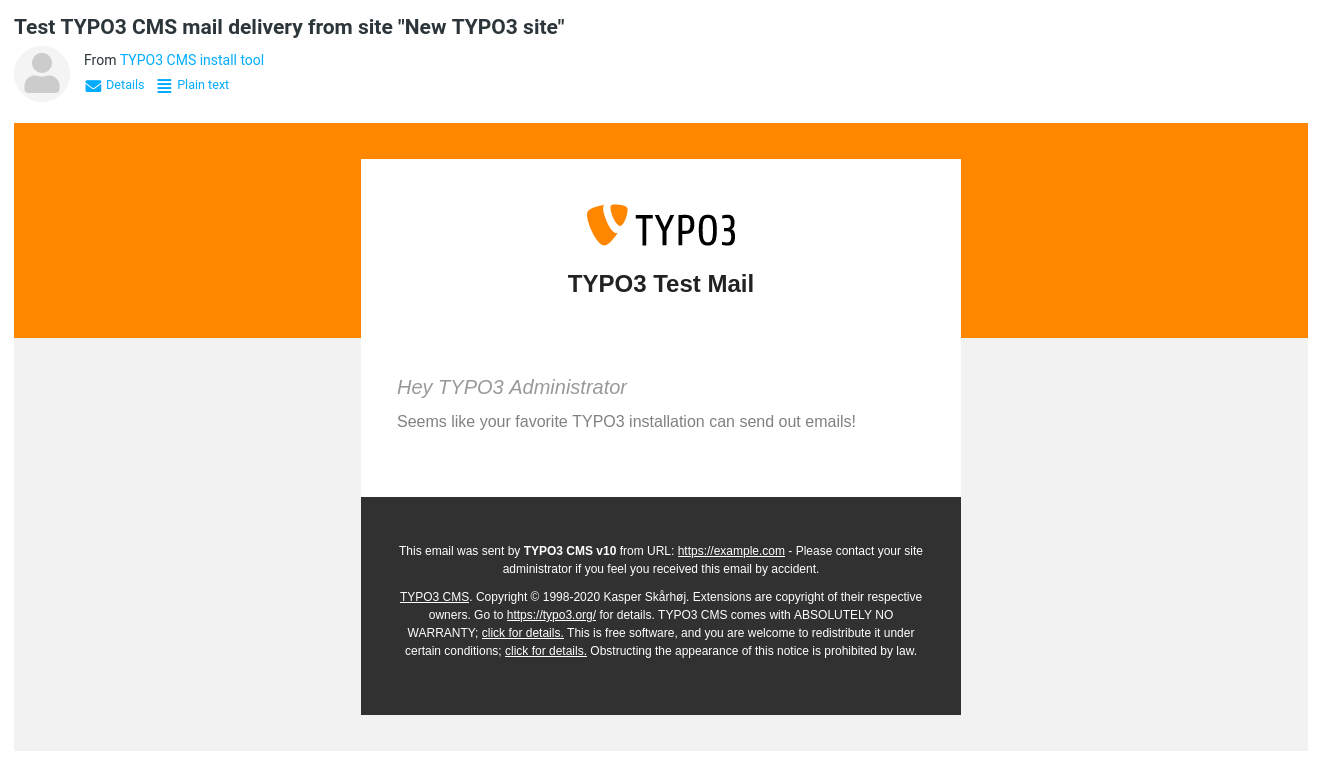
\includegraphics[width=0.8\linewidth]{InDepthChanges/90266-FluidBasedTemplatedEmails.png}
	\end{figure}

\end{frame}

% ------------------------------------------------------------------------------
% Feature | 88962 | Re-implement old PIDupinRootline TypoScript condition

\begin{frame}[fragile]
	\frametitle{Systeemwijzigingen}
	\framesubtitle{TypoScript}

	% decrease font size for code listing
	\lstset{basicstyle=\smaller\ttfamily}

	\begin{itemize}
		\item De oude \texttt{PIDupinRootline} voorwaarde is opnieuw geïmplementeerd
			in TypoScript met de Symfony uitdrukkingstaal.
		\item Syntax van oude TypoScript voorwaarde:
\begin{lstlisting}
[PIDupinRootline = 30]
  page.10.value = Ik ben op een subpagina van pagina met UID 30.
[END]
\end{lstlisting}

		\item Nieuwe syntax TypoScript voorwaarde:
\begin{lstlisting}
[30 in tree.rootLineParentIds]
  page.10.value = Ik ben op een subpagina van pagina met UID 30.
[END]
\end{lstlisting}

	\end{itemize}

\end{frame}

% ------------------------------------------------------------------------------
% Feature | 90426 | Browser-native lazy loading for images

\begin{frame}[fragile]
	\frametitle{Systeemwijzigingen}
	\framesubtitle{Vertraagd laden van afbeeldingen}

	% decrease font size for code listing
	\lstset{basicstyle=\smaller\ttfamily}

	\begin{itemize}
		\item Het HTML attribuut \texttt{loading} kan ingesteld worden bij \texttt{<img>}-tags.
		\item Browsers die dit ondersteunen zullen de afbeeldingen pas laden als ze zichtbaar worden.
		\item Dit gedrag kan gewijzigd worden met de volgende TypoScript constante:
\begin{lstlisting}
styles.content.image.lazyLoading = lazy
\end{lstlisting}

		\item Geldige waarden zijn: \texttt{lazy} (default), \texttt{eager}, en \texttt{auto}.
		\item De Fluid \textit{Image-ViewHelper} ondersteunt ook vertraagd laden:
\begin{lstlisting}
<f:image src="{fileObject}" treatIdAsReference="true"
  loading="lazy" />
\end{lstlisting}

	\end{itemize}

\end{frame}

% ------------------------------------------------------------------------------
% Important | 89869 | Change lockIP default to disabled for both frontend and backend

\begin{frame}[fragile]
	\frametitle{Systeemwijzigingen}
	\framesubtitle{Standaard waarden voor \texttt{lockIP}/\texttt{lockIPv6}}

	% decrease font size for code listing
	\lstset{basicstyle=\smaller\ttfamily}

	\begin{itemize}
		\item De standaardinstellingen voor \texttt{lockIP} zijn veranderd.
		\item De volgende vier systeemvariabelen zijn nu standaard \textbf{uitgeschakeld}:

			\begin{itemize}
				\item \texttt{[FE]['lockIP']}
				\item \texttt{[FE]['lockIPv6']}
				\item \texttt{[BE]['lockIP']}
				\item \texttt{[BE]['lockIPv6']}
			\end{itemize}

		\item De oude standaardwaarden ("\texttt{4}" voor de backend en "\texttt{2}" voor de frontend)
			zorgden voor problemen bij bezoekers met IPv4 en IPv6 ondersteuning.

	\end{itemize}

\end{frame}

% ------------------------------------------------------------------------------
% Feature | 88147 | Add possibility to configure the path to sitemap xslFile

\begin{frame}[fragile]
	\frametitle{Systeemwijzigingen}
	\framesubtitle{SEO: \texttt{Sitemap.xsl}}

	% decrease font size for code listing
	\lstset{basicstyle=\tiny\ttfamily}

	\begin{itemize}
		\item Het standaardpad naar het bestand \texttt{Sitempa.xsl} van de systeemextensie
			\texttt{EXT:seo} kan nu aangepast worden:
\begin{lstlisting}
# Globaal voor alle sitemaps:
plugin.tx_seo.config.xslFile = EXT:myext/Resources/Public/CSS/mySite.xsl

# Voor alle sitemaps van een specifiek type:
plugin.tx_seo.config.<sitemapType>.sitemaps.xslFile = EXT:myext/Resources/Public/CSS/mySite.xsl

# Voor een specifieke sitemap:
plugin.tx_seo.config.<sitemapType>.sitemaps.<sitemap>.config.xslFile =
  EXT:myext/Resources/Public/CSS/mySite.xsl
\end{lstlisting}

		\item Het standaardpad is:\newline
			\smaller
				\texttt{EXT:seo/Resources/Public/CSS/Sitemap.xsl}
			\normalsize

	\end{itemize}

\end{frame}

% ------------------------------------------------------------------------------
% Feature | 82062 | Progress for Reference Index update on CLI

\begin{frame}[fragile]
	\frametitle{Systeemwijzigingen}
	\framesubtitle{Referentie-index}

	% decrease font size for code listing
	\lstset{basicstyle=\tiny\ttfamily}

	\begin{itemize}
		\item Bij het bijwerken van de referentie-index toont een balk de voortgang voor elke
			databasetabel.
	\end{itemize}

	\begin{figure}
		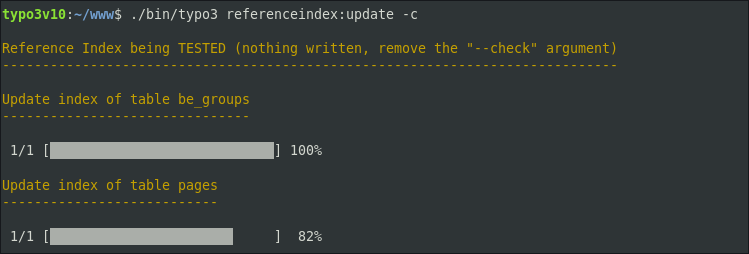
\includegraphics[width=0.85\linewidth]{InDepthChanges/82062-ProgressForReferenceIndexUpdateOnCli.png}
	\end{figure}

\end{frame}

% ------------------------------------------------------------------------------
% Feature | 59452 | scheduler:run command accepts multiple task options

\begin{frame}[fragile]
	\frametitle{Systeemwijzigingen}
	\framesubtitle{Taakplanner}

	% decrease font size for code listing
	\lstset{basicstyle=\tiny\ttfamily}

	\begin{itemize}
		\item Meerdere taken kunnen uitgevoerd worden met de optie \texttt{-}\texttt{-}\texttt{task}
	\end{itemize}

	\begin{figure}
		
\includegraphics[width=0.85\linewidth]{InDepthChanges/59452a-MultipleTasksInSchedulerCommand.png}
	\end{figure}

	\begin{itemize}
		\item Uitgebreide uitvoer kan ingeschakeld worden met \texttt{-}\texttt{v} en \texttt{-}\texttt{vv}
	\end{itemize}

	\begin{figure}
		
\includegraphics[width=0.85\linewidth]{InDepthChanges/59452b-MultipleTasksInSchedulerCommand.png}
	\end{figure}

\end{frame}

% ------------------------------------------------------------------------------
% Important | 18079 | pages.doktype restriction for frontend queries refined

\begin{frame}[fragile]
	\frametitle{Systeemwijzigingen}
	\framesubtitle{Paginatype afhandeling}

	\begin{itemize}
		\item Interne afhandeling van paginatypes is gewijzigd.
		\item De optie \texttt{pages.doktype} bepaalt een getal dat het type voorstelt,
			bijv. standaardpagina, map, snelkoppeling, link naar externe URL, enz.
		\item Pagina's van een bepaald type (bijv. map en prullenbak) waren uitgezonderd als inhoud
			werd gelezen uit een specifieke pagina of als records werden uitgelezen.
		\item De beperking is verwijderd en eigen paginatypes met een getal >200 zijn nu mogelijk.
		\item Integrators en ontwikkelaars die pagina doktypes hebben gebruikt, bijv. in TypoScript,
			wordt aangeraden te kijken of het oude gedrag werd misbruikt en nu bijgewerkt moet worden.
	\end{itemize}

\end{frame}

% ------------------------------------------------------------------------------
% Feature | 90203 | Make workspace available in TypoScript conditions

\begin{frame}[fragile]
	\frametitle{Systeemwijzigingen}
	\framesubtitle{Werkruimtes}

	% decrease font size for code listing
	\lstset{basicstyle=\smaller\ttfamily}

	\begin{itemize}
		\item Een nieuwe variabele voor de expressietaal is toegevoegd: \texttt{workspace}.
		\item Deze variabele kan in vergelijkingen gebruikt worden met gebruikelijke parameters van werkruimtes.
		\item Momenteel worden de volgende parameters ondersteund:\newline
			\small
				\texttt{workspaceId}, \texttt{isLive}, and \texttt{isOffline}.
			\normalsize
		\item Voorbeeld:
\begin{lstlisting}
[workspace.workspaceId === 3]
  # Huidige werkruimte ID is 3
[end]
\end{lstlisting}

	\end{itemize}

\end{frame}

% ------------------------------------------------------------------------------
% Important | 89555 | Workspace-related database records contain the proper Page ID

\begin{frame}[fragile]
	\frametitle{Systeemwijzigingen}
	\framesubtitle{Werkruimtes}

	\begin{itemize}
		\item Lange tijd gebruikte TYPO3 \texttt{pid} waarde \texttt{-1} voor ongepubliceerde records.
		\item TYPO3 bekijkt nu de volgende drie velden voor records in versiebeheer:

			\begin{itemize}
				\item \texttt{t3ver\_wsid} (ID van werkruimte waarin record zit)
				\item \texttt{t3ver\_state} (type van record in versiebeheer)
				\item \texttt{t3ver\_oid} (live-versie van een record)
			\end{itemize}

		\item Daarom is \texttt{pid=-1} niet meer vereist.
		\item De Upgrade Wizard zet alle \texttt{pid} velden om van records in versiebeheer
			naar de echte \texttt{pid} waarden.
		\item Nieuwe installaties hebben geen last van deze wijziging.

	\end{itemize}

\end{frame}

% ------------------------------------------------------------------------------
% Deprecation | 91030 | Runtime-Activated Packages

\begin{frame}[fragile]
	\frametitle{Systeemwijzigingen}
	\framesubtitle{Runtime-geactiveerde extensies}

	\begin{itemize}
		\item De volgende globale configuratie-optie is als \textbf{verouderd} aangemerkt:\newline
			\smaller
				\texttt{\$GLOBALS['TYPO3\_CONF\_VARS']['EXT']['runtimeActivatedPackages']}
			\normalsize
		\item Het gebruik van runtime-geactiveerde exensies vertraagt het systeem significant.
		\item Integrators wordt aangeraden om de nodige stappen te nemen als dergelijke waarschuwingen
			verschijnen in de verouderingslog:\newline
			\begingroup
				\fontsize{8}{10}
				\texttt{Support for runtime activated packages will be removed in TYPO3 v11.0.}
			\endgroup

	\end{itemize}

\end{frame}

% ------------------------------------------------------------------------------
% Breaking | 88376 | Removed obsolete pageNotFound_handling settings

\begin{frame}[fragile]
	\frametitle{Systeemwijzigingen}
	\framesubtitle{Afhandeling pagina niet gevonden}

	\begin{itemize}

		\item De volgende globale TYPO3 instellingen zijn verwijderd:

			\begin{itemize}
				\item {\fontsize{7}{8}\selectfont\texttt{\$GLOBALS['TYPO3\_CONF\_VARS']['FE']['pageNotFound\_handling']}}
				\item {\fontsize{7}{8}\selectfont\texttt{\$GLOBALS['TYPO3\_CONF\_VARS']['FE']['pageNotFound\_handling\_statheader']}}
				\item {\fontsize{7}{8}\selectfont\texttt{\$GLOBALS['TYPO3\_CONF\_VARS']['FE']['pageNotFound\_handling\_accessdeniedheader']}}
				\item {\fontsize{7}{8}\selectfont\texttt{\$GLOBALS['TYPO3\_CONF\_VARS']['FE']['pageUnavailable\_handling']}}
				\item {\fontsize{7}{8}\selectfont\texttt{\$GLOBALS['TYPO3\_CONF\_VARS']['FE']['pageUnavailable\_handling\_statheader']}}
			\end{itemize}

			\begin{itemize}\smaller
				\item[\ding{228}] De site-afhandeling die in TYPO3 v9 is ge\"{\i}ntroduceerd vervangt deze opties.
			\end{itemize}\normalsize

	\end{itemize}

\end{frame}

% ------------------------------------------------------------------------------
% Important | 87980 | Page Is Being Generated Message Has Been Removed

\begin{frame}[fragile]
	\frametitle{Systeemwijzigingen}
	\framesubtitle{Afhandeling pagina niet gevonden}

	\begin{itemize}

		\item De melding "\textit{Page is being generated}" en het bijbehorende tijdelijke
			HTTP 503 antwoord zijn verwijderd.
	\end{itemize}

	\begin{figure}
		
\includegraphics[width=0.70\linewidth]{InDepthChanges/87980-PageIsBeingGenerated.png}
	\end{figure}

	\begin{itemize}
		\item In plaats van het uitstellen van het werk en te wachten op de uiteindelijk pagina-inhoud wachten
			gelijktijdige requests nu gewoon tot de echte pagina-inhoud is gemaakt.
	\end{itemize}

\end{frame}

% ------------------------------------------------------------------------------
% Feature | 84262 | Update EXT:felogin to Extbase (long-term goal, not completed yet)
% Breaking | 88706 | Streamline felogin locallang keys
% Breaking | 88129 | Renamed felogin flexform fields

\begin{frame}[fragile]
	\frametitle{Systeemwijzigingen}
	\framesubtitle{Frontend-aanmelding: Extbase}

	\begin{itemize}
		\item De aanmelding voor frontend-gebruikers (\texttt{EXT:felogin}) is omgezet naar Extbase/Fluid.

		\item De volgende wijzigingen zijn ge\"{\i}mplementeerd:

		\begin{itemize}
			\item[\ding{202}] Prefix "\texttt{ll\_}" is verwijderd van locallang-sleutels.

				\begin{itemize}
					\item[\ding{228}] Werk TypoScript bij als er taallabels zijn overschreven en verwijder de prefix "\texttt{ll\_}".
				\end{itemize}

			\item[\ding{203}] Bestaande FlexForm structuren zijn bijgewerkt.

				\begin{itemize}
					\item[\ding{228}] Voer de Upgrade-assistent uit om de FLexForm-waarden te migreren.
				\end{itemize}

		\end{itemize}

	\end{itemize}

\end{frame}

% ------------------------------------------------------------------------------
% Breaking | 88583 | Database field sys_language.static_lang_isocode removed
% Deprecation | 88567 | $GLOBALS['LOCAL_LANG']

\begin{frame}[fragile]
	\frametitle{Systeemwijzigingen}
	\framesubtitle{Talen}

	\begin{itemize}
		\item ISO Codes:

			\begin{itemize}
				\item Het ongebruikte database-veld \texttt{static\_lang\_isocode} is verwijderd.
				\item \texttt{EXT:static\_info\_tables} kan worden ge\"{\i}nstalleerd om de functionaliteit te herintroduceren.
				\item Ontwikkelaars wordt aangeraden alle metadata van een taal uit de Site Configuration en de SiteLanguage API te halen.
			\end{itemize}

		\item Taalbestanden:

			\begin{itemize}
				\item Gebruik van de globale array \texttt{\$GLOBALS[LOCAL\_LANG]} is als verouderd aangemerkt.
				\item Het 2e en 3e argument van \texttt{LanguageService->includeLLFile()} is als verouderd aangemerkt.
			\end{itemize}

	\end{itemize}

\end{frame}

% ------------------------------------------------------------------------------
% Feature | 88643 | New Mail API based on symfony/mailer and symfony/mime
% Breaking | 88643 | Removed Swiftmailerswiftmailer Dependency

\begin{frame}[fragile]
	\frametitle{Systeemwijzigingen}
	\framesubtitle{Nieuwe E-mail-API}

	\begin{itemize}
		\item SwiftMailer is opgevolgd door modernere bibliotheken:

			\begin{itemize}
				\item \texttt{symfony/mime} voor het maken e-mailberichten
				\item \texttt{symfony/mailer} voor het versturen van e-mails
			\end{itemize}

		\item PHP functie \texttt{mail()} wordt niet langer ondersteund.

			\begin{itemize}\smaller
				\item[\ding{228}] Aangeraden wordt om \texttt{sendmail} of \texttt{smtp} te gebruiken.
			\end{itemize}\normalsize

		\item Maatwerk SwiftMailer plug-ins of transports vergen migratie.

		\item Zie de \href{https://symfony.com/doc/current/mailer.html}{Symfony Documentatie}
			voor meer details hoe de nieuwe E-mail API te gebruiken.
	\end{itemize}

\end{frame}

% ------------------------------------------------------------------------------
% ...

\begin{frame}[fragile]
	\frametitle{Systeemwijzigingen}
	\framesubtitle{PSR-standaarden}

	\begin{itemize}
		\item TYPO3 v10 LTS volgt deze \href{https://www.php-fig.org/psr/}{PSR-standaarden}:
			\vspace{0.2cm}
			\begin{itemize}
				\item PSR-0 / PSR-4\tabto{3.7cm}Autoloading
				\item PSR-1 / PSR-2\tabto{3.7cm}Coding Standards
				\item PSR-3\tabto{3.7cm}Logging
				\item PSR-7 / PSR-15 / PSR-17\tabto{3.7cm}HTTP Request / Response handling)
				\item PSR-11\tabto{3.7cm}Dependency Injection (Service Container)
				\item PSR-14\tabto{3.7cm}Event Dispatcher
				\item PSR-18\tabto{3.7cm}HTTP Client
			\end{itemize}

	\end{itemize}

\end{frame}

% ------------------------------------------------------------------------------
% Feature | 88799 | Use PSR-3 interface for logging

\begin{frame}[fragile]
	\frametitle{Systeemwijzigingen}
	\framesubtitle{PSR-3 koppelvlak voor logs}

	\begin{itemize}
		\item het TYPO3 Logging Framework (speciaal LogLevel en LogManager) gebruiken nu het
			\href{https://www.php-fig.org/psr/psr-3/}{PSR-3 Koppelvlak voor logs}.

		\item PSR-3 is een standaardmethode waarbij bibliotheken een
			\texttt{Psr\textbackslash
				Log\textbackslash
				LoggerInterface} object ontvangen en op een simpele en universele manier
				naar logs kunnen schrijven.

			\item Hiermee kunnen Ontwikkelaars eigen logs gebruiken en gebuik maken van
				andere logsystemen.

	\end{itemize}

\end{frame}

% ------------------------------------------------------------------------------
% Feature | 84112 | Symfony dependency injection for core and Extbase

\begin{frame}[fragile]
	\frametitle{Systeemwijzigingen}
	\framesubtitle{PSR-11 Symfony afhankelijkheidsinjectie}

	\begin{itemize}
		\item Het pakket \texttt{symfony/dependency-injection} is ge\"{\i}ntegreerd
			en wordt gebruikt om in het hele systeem afhankelijkheden te beheren en
			te injecteren in klassen.

		\item Met deze benadering moet uiteindelijk de Extbase injectiecontainer en
			en de objectbeheerder vervangen worden.

		\item Daarom moeten klassen aangepast worden en indien mogelijk vermeden:

			\begin{itemize}\small
				\item \texttt{\textbackslash
					TYPO3\textbackslash
					CMS\textbackslash
					Extbase\textbackslash
					Object\textbackslash
					ObjectManager}
				\item \texttt{\textbackslash
					TYPO3\textbackslash
					CMS\textbackslash
					Core\textbackslash
					Utility\textbackslash
					GeneralUtility::makeInstance()}
			\end{itemize}\normalsize

	\end{itemize}

\end{frame}

% ------------------------------------------------------------------------------
% Feature | 84112 | Symfony dependency injection for core and Extbase

\begin{frame}[fragile]
	\frametitle{Systeemwijzigingen}
	\framesubtitle{PSR-11 Symfony afhankelijkheidsinjectie}

	% decrease font size for code listing
	\lstset{basicstyle=\tiny\ttfamily}

	\begin{itemize}
		\item Configuratie-opties omvatten:

			\begin{itemize}
				\item Autobedrading (zie voorbeeld hieronder)
				\item Handmatige bedrading
					(zie \href{https://docs.typo3.org/c/typo3/cms-core/master/en-us/Changelog/10.0/Feature-84112-SymfonyDependencyInjectionForCoreAndExtbase.html}{lijst wijzigingen})
				\item Uitgebreide functionaliteit
					(zie \href{https://docs.typo3.org/c/typo3/cms-core/master/en-us/Changelog/10.0/Feature-84112-SymfonyDependencyInjectionForCoreAndExtbase.html}{lijst wijzigingen})
			\end{itemize}
\begin{lstlisting}
# Configuration/Services.yaml
services:
  _defaults:
    autowire: true
    autoconfigure: true
    public: false

  Your\Namespace\:
    resource: '../Classes/*'
\end{lstlisting}

		\item Zie \href{https://symfony.com/doc/current/service_container.html}{Symfony documentatie} voor meer details.

	\end{itemize}

\end{frame}

% ------------------------------------------------------------------------------
% Feature | 88769 | Introduce a generic EventDispatcher based on PSR-14
% Feature | 88770 | Add PSR-14 EventDispatcher logic based on DI

\begin{frame}[fragile]
	\frametitle{Systeemwijzigingen}
	\framesubtitle{PSR-14 Afwikkeling gebeurtenissen}

	\begin{itemize}
		\item Een nieuw systeem voor het afhandelen van gebeurtenissen is toegevoegd en zal
			de hooks en signal/slot concepten vervangen.

		\item Het is gebaseerd op de \href{https://www.php-fig.org/psr/psr-14}{PSR-14 standaard}
			waarmee ontwikkelaars op een simpele en consistente manier logica kunnen injecteren in een applicatie.

		\item PSR-14 bestaat uit de volgende vier onderdelen:

			\begin{itemize}
				\item Een \textbf{EventDispatcher} object waarmee je een gebeurtenis activeert.
				\item Een \textbf{ListenerProvider} object dat geregistreerde luisteraars voor alle gebeurtenissen bevat.
				\item Een of meerdere \textbf{Event} objecten die vanuit TYPO3 of extensies ("Emitter") aangeroepen worden.
				\item Een of meerdere \textbf{Listeners} (normaliter in extensies of PHP pakketten) die zijn geregistreerd.
			\end{itemize}

% Short-Term goal is to deprecate SignalSlot dispatcher in TYPO3 v10,
% and migrate all signals to the EventDispatcher.

	\end{itemize}

\end{frame}

% ------------------------------------------------------------------------------
% Feature | 88769 | Introduce a generic EventDispatcher based on PSR-14
% Feature | 88770 | Add PSR-14 EventDispatcher logic based on DI

\begin{frame}[fragile]
	\frametitle{Systeemwijzigingen}
	\framesubtitle{PSR-14 Afwikkeling gebeurtenissen}

	% decrease font size for code listing
	\lstset{basicstyle=\tiny\ttfamily}

	Voorbeeld implementatie

	\begin{itemize}\smaller
		\item[\ding{202}] Voeg \texttt{event.listener} label toe aan bestand \texttt{Configuration/Services.yaml}:
\begin{lstlisting}
services:
  Vendor\Example\EventListener\NullMailer:
    tags:
      - { name: event.listener, identifier: 'myListener', event: TYPO3\CMS\Core\Mail\Event\AfterMailerInitializationEvent, before: 'redirects, anotherIdentifier' }
\end{lstlisting}

		\item[\ding{203}] Implementeer het event object:
\begin{lstlisting}
namespace Vendor\Example\EventListener;

class NullMailer
{
  public function __invoke(AfterMailerInitializationEvent $event): void
  {
    $event->getMailer()->injectMailSettings(['transport' => 'null']);
  }
}
\end{lstlisting}

	\end{itemize}\normalsize

\end{frame}

% ------------------------------------------------------------------------------
% Feature | 88769 | Introduce a generic EventDispatcher based on PSR-14
% Feature | 88770 | Add PSR-14 EventDispatcher logic based on DI

\begin{frame}[fragile]
	\frametitle{Systeemwijzigingen}
	\framesubtitle{PSR-14 Afwikkeling gebeurtenissen}

	% decrease font size for code listing
	\lstset{basicstyle=\tiny\ttfamily}

	\begin{itemize}
		\item Lijst met beschikbare Event Listeners is beschikbaar in de backend:\newline
			\smaller
				(vereist systeemextensies \texttt{EXT:lowlevel})
			\normalsize
	\end{itemize}

	\begin{figure}
		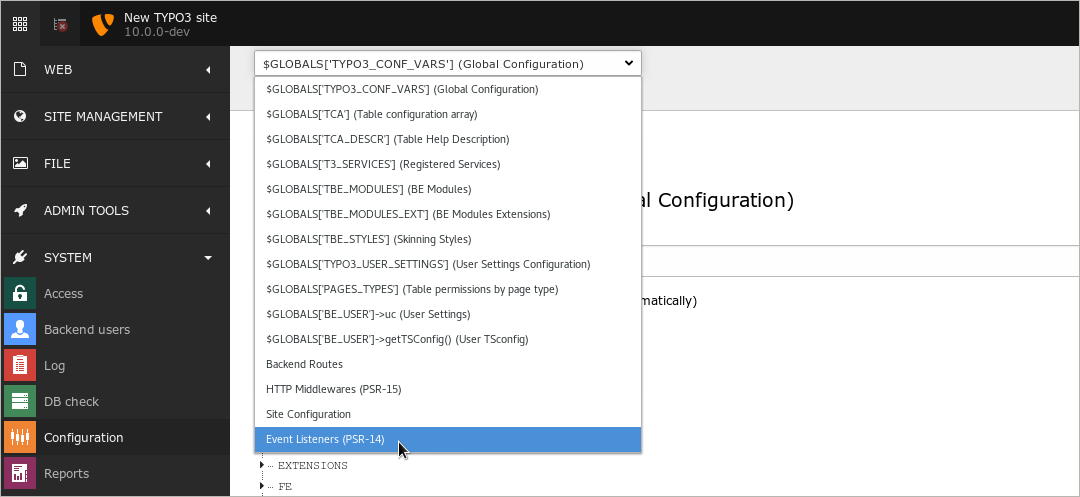
\includegraphics[width=0.70\linewidth]{InDepthChanges/88770-PSR14-EventDispatcher.png}
	\end{figure}

\end{frame}

% ------------------------------------------------------------------------------
% Feature | 88769 | Introduce a generic EventDispatcher based on PSR-14
% Feature | 88770 | Add PSR-14 EventDispatcher logic based on DI

\begin{frame}[fragile]
	\frametitle{Systeemwijzigingen}
	\framesubtitle{PSR-14 Afwikkeling gebeurtenissen}

	% decrease font size for code listing
	\lstset{basicstyle=\tiny\ttfamily}

	\begin{itemize}
		\item Aanbevolen methode:

			\begin{itemize}
				\item Voeg slechts één Listener per PHP klasse toe en gebruik \texttt{\_\_invoke()} als functienaam.
				\item Voeg "\texttt{Event}" achtervoegsel toe aan klassenaam bij een nieuwe Event klasse.
				\item Zet het Event PHP klassebestand in een geschikte map, bijv. \texttt{Classes/Database/Event}.
				\item Gebruik afhankelijkheidsinjectie in de vorm van een constructor-argument om indien nodig
					het EventDispatcher object te ontvangen.
			\end{itemize}

		\item Extra opmerking:\newline
			\small
				Gebeurtenissen die de TYPO3 core biedt volgen het beleid voor veroudering, behalve voor de constructor-argumenten
				die wel kunnen wijzigen.
			\normalsize

	\end{itemize}

\end{frame}

% ------------------------------------------------------------------------------
% Feature | 90265 | Show dispatched Events in Admin Panel

\begin{frame}[fragile]
	\frametitle{Systeemwijzigingen}
	\framesubtitle{PSR-14 Events in Admin Panel}

	\begin{itemize}
		\item Het Admin Panel toont alle PSR-14 events die in het huidige pagina zijn aangeroepen.
	\end{itemize}

	\begin{figure}
		
\includegraphics[width=0.85\linewidth]{InDepthChanges/90265-ShowDispatchedEventsInAdminPanel.png}
	\end{figure}

\end{frame}

% ------------------------------------------------------------------------------
% Feature | 89018 | Provide implementation for PSR-17 HTTP Message Factories

\begin{frame}[fragile]
	\frametitle{Systeemwijzigingen}
	\framesubtitle{PSR-17 HTTP Message Factories}

	\begin{itemize}
		\item De \href{https://www.php-fig.org/psr/psr-17/}{PSR-17}
			HTTP Message Factories implementatie is toegevoegd.
		\item HTTP Message Factory koppelvlakken zouden als afhankelijkheden gebruikt worden voor
			request handlers of services die PSR-7 berichtobjecten aanmaken.
		\item PSR-17 bevat zes factory-koppelvlakken:

			\begin{itemize}\smaller
				\item \texttt{\textbackslash
					Psr\textbackslash
					Http\textbackslash
					Message\textbackslash
					RequestFactoryInterface}
				\item \texttt{\textbackslash
					Psr\textbackslash
					Http\textbackslash
					Message\textbackslash
					ResponseFactoryInterface}
				\item \texttt{\textbackslash
					Psr\textbackslash
					Http\textbackslash
					Message\textbackslash
					ServerRequestFactoryInterface}
				\item \texttt{\textbackslash
					Psr\textbackslash
					Http\textbackslash
					Message\textbackslash
					StreamFactoryInterface}
				\item \texttt{\textbackslash
					Psr\textbackslash
					Http\textbackslash
					Message\textbackslash
					UploadedFileFactoryInterface}
				\item \texttt{\textbackslash
					Psr\textbackslash
					Http\textbackslash
					Message\textbackslash
					UriFactoryInterface}

			\end{itemize}\normalsize

		\item Zie
			\href{https://docs.typo3.org/c/typo3/cms-core/master/en-us/Changelog/10.1/Feature-89018-ProvideImplementationForPSR-17HTTPMessageFactories.html}{documentatie}
			voor voorbeeldcode.

	\end{itemize}

\end{frame}

% ------------------------------------------------------------------------------
% Feature | 89216 | PSR-18 HTTP Client Implementation

\begin{frame}[fragile]
	\frametitle{Systeemwijzigingen}
	\framesubtitle{PSR-18 HTTP Client}

	\begin{itemize}
		\item De \href{https://www.php-fig.org/psr/psr-18/}{PSR-18}
			HTTP Client implementatie is toegevoegd.
		\item Hiermee kunnen ontwikkelaars HTTP request gebaseerd op PSR-7 berichtobjecten
			maken zonder af te hangen van een specifieke implementatie van een HTTP client.
		\item Het vervangt niet de bestaande \href{http://guzzlephp.org/}{Guzzle}
			functies maar biedt een meer generiek alternatief.
		\item PSR-18 bestaat uit een clientkoppelvlak en drie uitzonderingskoppelvlakken:

			\begin{itemize}\smaller
				\item \texttt{\textbackslash
					Psr\textbackslash
					Http\textbackslash
					Client\textbackslash
					ClientInterface}
				\item \texttt{\textbackslash
					Psr\textbackslash
					Http\textbackslash
					Client\textbackslash
					ClientExceptionInterface}
				\item \texttt{\textbackslash
					Psr\textbackslash
					Http\textbackslash
					Client\textbackslash
					NetworkExceptionInterface}
				\item \texttt{\textbackslash
					Psr\textbackslash
					Http\textbackslash
					Client\textbackslash
					RequestExceptionInterface}
			\end{itemize}\normalsize

		\item Zie
			\href{https://docs.typo3.org/c/typo3/cms-core/master/en-us/Changelog/10.1/Feature-89216-PSR-18HTTPClientImplementation.html}{documentatie}
			voor een codevoorbeeld.

	\end{itemize}

\end{frame}

% ------------------------------------------------------------------------------
% Breaking | 88182 | jsfunc.inline.js has been dropped
% Breaking | 88427 | jsfunc.evalfield.js has been removed
% Breaking | 88667 | Removed additionalJavaScriptSubmit from FormEngine
% Deprecation | 88433 | Deprecate top.openUrlInWindow

\begin{frame}[fragile]
	\frametitle{Systeemwijzigingen}
	\framesubtitle{JavaScript opties en functies}

	\begin{itemize}
		\item De volgende JavaScript-bestanden zijn verwijderd:

			\begin{itemize}
				\item \texttt{jsfunc.inline.js}
				\item \texttt{jsfunc.evalfield.js}
			\end{itemize}

			\begin{itemize}\smaller
				\item[\ding{228}] Gebruik \texttt{TYPO3/CMS/Backend/FormEngineValidation} in plaats daarvan.
			\end{itemize}\normalsize

		\item Extra submit-handlers kunnen voorheen zijn toegevoegd met de optie \texttt{additionalJavaScriptSubmit}.
			Deze optie is verwijderd.

			\begin{itemize}\smaller
				\item[\ding{228}] Maak en registreer in plaats hiervan een AMD module.
			\end{itemize}\normalsize

		\item De globale JavaScript-functie \texttt{top.openUrlInWindow()} is als verouderd aangemerkt.

	\end{itemize}

\end{frame}

% ------------------------------------------------------------------------------
% Breaking | 88411 | TBE_EDITOR.typo3form removed
% Deprecation | 88432 | Replaced md5js with an AMD module
% Deprecation | 88428 | top.rawurlencode and top.str_replace
% Deprecation | 88651 | Replace TYPO3/CMS/Backend/SplitButtons with TYPO3/CMS/Backend/DocumentSaveActions

\begin{frame}[fragile]
	\frametitle{Systeemwijzigingen}
	\framesubtitle{JavaScript opties en functies}

	\begin{itemize}

		\item Het globale object \texttt{TBE\_EDITOR.typo3form} en z'n achterliggende lagen \texttt{typo3FormFieldSet}
			en \texttt{typo3FormFieldGet} zijn verwijderd.

		\item Bestand \texttt{md5.js} is als verouderd aangemerkt.

			\begin{itemize}\smaller
				\item[\ding{228}] Laad in plaats hiervan de AMD module \texttt{TYPO3/CMS/Backend/Hashing/Md5} via RequireJS.
			\end{itemize}\normalsize

		\item De volgende globale JavaScript-functies zijn als verouderd aangemerkt:

			\begin{itemize}
				\item \texttt{top.rawurlencode()}
				\item \texttt{top.str\_replace()}
			\end{itemize}

		\item Module \texttt{TYPO3/CMS/Backend.SplitButtons} is als verouderd aangemerkt.

			\begin{itemize}\smaller
				\item[\ding{228}] Gebruik in plaats hiervan \texttt{TYPO3/CMS/Backend/DocumentSaveActions}.
			\end{itemize}\normalsize

 	\end{itemize}

\end{frame}

% ------------------------------------------------------------------------------
% Important | 87894 | Removed PHP Dependency algo26-matthiasidna-convert

\begin{frame}[fragile]
	\frametitle{Systeemwijzigingen}
	\framesubtitle{UTF-8-gebaseerde domeinen}

	\begin{itemize}
		\item PHP heeft eigen functies om domeinen van UTF-8 naar IDNA ASCII formaat (“punicode”) om te zetten,
			bijv. \href{https://www.php.net/manual/en/function.idn-to-ascii.php}{idn\_to\_ascii()}.

		\item Deze kunnen direct gebruikt worden als de PHP extensie
			"\href{https://www.php.net/manual/en/book.intl.php}{intl}" aanwezig is.

		\item Als de PHP extensie niet aanwezig is biedt het pakket \texttt{symfony/polyfill-intl-idn}
			nu de functies.

		\item Hiervoor werd het pakket \texttt{algo26-matthias/idna-convert} gebruikt en deze is nu verwijderd.

	\end{itemize}

\end{frame}

% ------------------------------------------------------------------------------
% Feature | 87665 | Introduce BitSet class

\begin{frame}[fragile]
	\frametitle{Systeemwijzigingen}
	\framesubtitle{BitSet Class}

	% decrease font size for code listing
	\lstset{basicstyle=\tiny\ttfamily}

	\begin{itemize}
		\item Een nieuwe klasse is beschikbaar voor het efficiënt gebruiken van booleaanse vlaggen:\newline
			\texttt{TYPO3\textbackslash
				CMS\textbackslash
				Core\textbackslash
				Type\textbackslash
				BitSet}

		\item For example:
\begin{lstlisting}
define('PERMISSIONS_NONE', 0b0); // 0
define('PERMISSIONS_PAGE_SHOW', 0b1); // 1
define('PERMISSIONS_PAGE_EDIT', 0b10); // 2
define('PERMISSIONS_PAGE_DELETE', 0b100); // 4
define('PERMISSIONS_PAGE_NEW', 0b1000); // 8
define('PERMISSIONS_CONTENT_EDIT', 0b10000); // 16
define('PERMISSIONS_ALL', 0b11111); // 31

$bitSet = new \TYPO3\CMS\Core\Type\BitSet(PERMISSIONS_PAGE_SHOW | PERMISSIONS_PAGE_NEW);
$bitSet->get(PERMISSIONS_PAGE_SHOW); // true
$bitSet->get(PERMISSIONS_CONTENT_EDIT); // false
\end{lstlisting}

	\end{itemize}

\end{frame}

% ------------------------------------------------------------------------------
% Important | 87516 | Remove Core HTTP Request Handler Interface

\begin{frame}[fragile]
	\frametitle{Systeemwijzigingen}
	\framesubtitle{Request Handler}

	\begin{itemize}
		\item Het volgende interne koppelvlak is verwijderd en vervangen door
			koppelvlakken van PSR-15 request handler en middleware:\newline
			\texttt{TYPO3\textbackslash
				CMS\textbackslash
				Core\textbackslash
				Http\textbackslash
				RequestHandlerInterface}

	\end{itemize}

\end{frame}

% ------------------------------------------------------------------------------
% Breaking | 88687 | Configure extbase request handlers via PHP

\begin{frame}[fragile]
	\frametitle{Systeemwijzigingen}
	\framesubtitle{Request Handler}

	% decrease font size for code listing
	\lstset{basicstyle=\tiny\ttfamily}

	\begin{itemize}
		\item De configuratie van Extbase request handlers is niet langer mogelijk met TypoScript.

		\smaller\textbf{Oude} methode in TypoScript:\normalsize
\begin{lstlisting}
config.tx_extbase {
  mvc {
    requestHandlers {
      Vendor\Example\Mvc\Web\FrontendRequestHandler = Vendor\Example\Mvc\Web\FrontendRequestHandler
    }
  }
}
\end{lstlisting}

		\smaller\textbf{Nieuwe} methode in bestand \texttt{Configuration/Extbase/RequestHandlers.php}:\normalsize
\begin{lstlisting}
<?php
declare(strict_types = 1);

return [
  \Vendor\Example\Mvc\Web\FrontendRequestHandler::class,
];
\end{lstlisting}

	\end{itemize}

\end{frame}

% ------------------------------------------------------------------------------
% Deprecation | 87550 | Use controller classes when registering plugins/modules

\begin{frame}[fragile]
	\frametitle{Systeemwijzigingen}
	\framesubtitle{Extbase en Fluid}

	% decrease font size for code listing
	\lstset{basicstyle=\tiny\ttfamily}

	\begin{itemize}
		\item Het registreren van plug-ins/modules vergt nu volledige klassenamen

			\begin{itemize}\smaller
				\item \texttt{\textbackslash
					TYPO3\textbackslash
					CMS\textbackslash
					Extbase\textbackslash
					Utility\textbackslash
					ExtensionUtility::configurePlugin()}
				\item \texttt{\textbackslash
					TYPO3\textbackslash
					CMS\textbackslash
					Extbase\textbackslash
					Utility\textbackslash
					ExtensionUtility::registerModule()}
			\end{itemize}\normalsize

		\item Laat ook de vendor naam weg in de naam van de extensie (eerste argument).

			\begin{itemize}\smaller
				\item[\ding{228}] Gebruik "\texttt{ExampleBlog}" in plaats van "\texttt{Vendor.ExampleBlog}".
			\end{itemize}

		\item Bijvoorbeeld:
\begin{lstlisting}
\TYPO3\CMS\Extbase\Utility\ExtensionUtility::configurePlugin(
  'ExampleBlog', // previously: 'Vendor.ExampleBlog'
  'pi1',
  [
    \Vendor\Example\Controller\BlogController::class => 'list,update,delete'
  ],
  [
    \Vendor\Example\Controller\BlogController::class => 'list,update,delete'
  ]
);
\end{lstlisting}

	\end{itemize}

\end{frame}

% ------------------------------------------------------------------------------
% Breaking | 87627 | Remove Property extensionName of AbstractController

\begin{frame}[fragile]
	\frametitle{Systeemwijzigingen}
	\framesubtitle{Extbase en Fluid}

	\begin{itemize}
		\item Eigenschap \texttt{extensionName} van AbstractController is verwijderd.

			\begin{itemize}\smaller
				\item[\ding{228}] Gebruik \texttt{\textbackslash
					TYPO3\textbackslash
					CMS\textbackslash
					Extbase\textbackslash
					Mvc\textbackslash
					Request::getControllerExtensionName()} in plaats daarvan.
			\end{itemize}\normalsize

	\end{itemize}

\end{frame}

% ------------------------------------------------------------------------------
% Feature | 87457 | Use symfony/propertyinfo to gather doc block information

\begin{frame}[fragile]
	\frametitle{Systeemwijzigingen}
	\framesubtitle{Extbase en Fluid}

	% decrease font size for code listing
	\lstset{basicstyle=\tiny\ttfamily}

	\begin{itemize}
		\item Extbase modellen ondersteunen nu afgekorte klassenamen in Doc-blokken.
\begin{lstlisting}
use TYPO3\CMS\Extbase\Persistence\ObjectStorage;
use ExtbaseTeam\BlogExample\Domain\Model\Comment;

class Post
{
  /**
   * @var ObjectStorage<Comment>
   */
  public $comments;
}
\end{lstlisting}

	\end{itemize}

\end{frame}

% ------------------------------------------------------------------------------
% Breaking | 87957 | Validators are not registered automatically in Extbase anymore

\begin{frame}[fragile]
	\frametitle{Systeemwijzigingen}
	\framesubtitle{Extbase en Fluid}

	% decrease font size for code listing
	\lstset{basicstyle=\tiny\ttfamily}

	\begin{itemize}
		\item Validators worden niet meer automatisch geregistreerd in Extbase.
		\item Voor een model met de naam
			\small\texttt{Vendor\textbackslash
				Example\textbackslash
				Domain\textbackslash
				Model\textbackslash
				Blog}\normalsize,\newline
			gebruikte Extbase automatisch de validator
			\small\texttt{Vendor\textbackslash
				Example\textbackslash
				Domain\textbackslash
				Validator\textbackslash
				BlogValidator}\normalsize

		\item Validators moeten nu handmatig geregistreerd worden:
\begin{lstlisting}
use Vendor\Example\Domain\Model\Blog;
use TYPO3\CMS\Extbase\Annotation as Extbase;
use TYPO3\CMS\Extbase\Mvc\Controller\ActionController;

class BlogController extends ActionController
{
  /**
   * @Extbase\Validate(param="blog", validator="Vendor\Example\Domain\Validator\BlogValidator")
   */
  public function showAction(Blog $blog)
  {
    // ...
  }
}
\end{lstlisting}

	\end{itemize}

\end{frame}

% ------------------------------------------------------------------------------
% Breaking | 87594 | Harden Extbase

\begin{frame}[fragile]
	\frametitle{Systeemwijzigingen}
	\framesubtitle{Extbase en Fluid}

	% decrease font size for code listing
	\lstset{basicstyle=\smaller\ttfamily}

	\begin{itemize}
		\item Klassen gebruiken nu de "strict type" modus en type-hints voor scalaire parameters
\begin{lstlisting}
<?php
declare(strict_types = 1);
\end{lstlisting}

		% Method signatures in Extbase classes have been updated.
		\item Dit geeft fatale PHP-fouten als de definitie van een functie in maatwerk
			extensies niet overeenkomt met interfaces en/of bovenliggende klassen.

		\item Zie \href{https://forge.typo3.org/issues/87594}{forge \#87594}
			voor een complete lijst van bestanden en hun wijzigingen.

		\item Dit is nog werk in uitvoering en verdere aanpassingen volgen.

	\end{itemize}

\end{frame}

% ------------------------------------------------------------------------------
% Feature | 88995 | Calling registerPlugin with vendor name

\begin{frame}[fragile]
	\frametitle{Systeemwijzigingen}
	\framesubtitle{Extbase en Fluid}

	% decrease font size for code listing
	\lstset{basicstyle=\smaller\ttfamily}

	\begin{itemize}
		\item Laat de vendor weg bij het registreren van plug-ins met\newline
			\smaller
				\texttt{\textbackslash
					TYPO3\textbackslash
					CMS\textbackslash
					Extbase\textbackslash
					Utility\textbackslash
					ExtensionUtility::registerPlugin()}
			\normalsize

		\item Bijv., gebruik "\texttt{Form}" in plaats van "\texttt{TYPO3.CMS.Form}"\newline
			\small(eerste parameter)\normalsize
\begin{lstlisting}
\TYPO3\CMS\Extbase\Utility\ExtensionUtility::registerPlugin(
  'Form',
  'Formframework',
  'Form',
  'content-form',
);
\end{lstlisting}

	\end{itemize}

\end{frame}

% ------------------------------------------------------------------------------
% Feature | 89870 | New PSR-14 Events for Extbase-related signals

\begin{frame}[fragile]
	\frametitle{Systeemwijzigingen}
	\framesubtitle{Extbase en Fluid}

	% decrease font size for code listing
	\lstset{basicstyle=\tiny\ttfamily}

	\begin{itemize}
		\item De volgende PSR-14-gebaseerde events zijn toegevoegd aan signals in Extbase:
\begin{lstlisting}
TYPO3\CMS\Extbase\Event\Mvc\AfterRequestDispatchedEvent
TYPO3\CMS\Extbase\Event\Mvc\BeforeActionCallEvent
TYPO3\CMS\Extbase\Event\Persistence\AfterObjectThawedEvent
TYPO3\CMS\Extbase\Event\Persistence\ModifyQueryBeforeFetchingObjectDataEvent
TYPO3\CMS\Extbase\Event\Persistence\ModifyResultAfterFetchingObjectDataEvent
TYPO3\CMS\Extbase\Event\Persistence\EntityAddedToPersistenceEvent
TYPO3\CMS\Extbase\Event\Persistence\EntityFinalizedAfterPersistenceEvent
TYPO3\CMS\Extbase\Event\Persistence\EntityUpdatedInPersistenceEvent
TYPO3\CMS\Extbase\Event\Persistence\EntityRemovedFromPersistenceEvent
TYPO3\CMS\Extbase\Event\Persistence\EntityPersistedEvent
\end{lstlisting}

		\item Bestaande signals zijn vervangen en moeten niet meer gebruikt worden.

	\end{itemize}

\end{frame}

% ------------------------------------------------------------------------------
% Breaking | 87623 | Replace config.persistence.classes typoscript configuration (1)

\begin{frame}[fragile]
	\frametitle{Systeemwijzigingen}
	\framesubtitle{Extbase en Fluid - Mappen van klassen}

	% decrease font size for code listing
	\lstset{basicstyle=\tiny\ttfamily}

	\begin{itemize}
		\item Het mappen van klassen met TypoScript voor opslag is niet langer ondersteund:
\begin{lstlisting}
config.tx_example_blog {
  persistence {
    classes {
      Vendor\Example\Domain\Model\Author {
        mapping {
          tableName = fe_users
          columns.name.mapOnProperty = fullname
        }
      }
    }
  }
}
\end{lstlisting}

	\end{itemize}

\end{frame}

% ------------------------------------------------------------------------------
% Breaking | 87623 | Replace config.persistence.classes typoscript configuration (2)

\begin{frame}[fragile]
	\frametitle{Systeemwijzigingen}
	\framesubtitle{Extbase and Fluid - Class Mapping}

	% decrease font size for code listing
	\lstset{basicstyle=\tiny\ttfamily}

	\begin{itemize}
		\item Het mappen moet nu plaatsvinden in een PHP-bestand \texttt{Configuration/Extbase/Persistence/Classes.php}:
\begin{lstlisting}
<?php
declare(strict_types = 1);

return [
  \Vendor\Example\Domain\Model\Author::class => [
    'tableName' => 'fe_users',
    'properties' => [
      'fullname' => [
        'fieldName' => 'name'
      ]
    ]
  ]
];
\end{lstlisting}

		\begin{itemize}\smaller
			\item[\ding{228}] Let op: de naam van de eigenschap en het databaseveld zijn gewisseld!\newline
				Voorheen:\tabto{1.6cm}\texttt{<db-field>.mapOnProperty = <property>}\newline
				Nieuw:\tabto{1.6cm}\texttt{properties.<property>.fieldname = <db-field>}
		\end{itemize}\normalsize

	\end{itemize}

\end{frame}

% ------------------------------------------------------------------------------
% Deprecation | 88406 | setCacheHash/noCacheHash options in ViewHelpers and UriBuilder

\begin{frame}[fragile]
	\frametitle{Systeemwijzigingen}
	\framesubtitle{cHash in UriBuilder en ViewHelpers}

	% decrease font size for code listing
	\lstset{basicstyle=\smaller\ttfamily}

	\begin{itemize}
		\item De volgende twee Extbase UriBuilder functies zijn als verouderd aangemerkt:

			\begin{itemize}
				\item \texttt{UriBuilder->setUseCacheHash()}
				\item \texttt{UriBuilder->getUseCacheHash()}
			\end{itemize}

		\item Dit heeft ook impact op een aantal Fluid ViewHelpers:
	\end{itemize}
	\begin{columns}[T]
		\begin{column}{.05\textwidth}
		\end{column}
		\begin{column}{.45\textwidth}
			\begin{itemize}\smaller
				\item \texttt{f:form}
				\item \texttt{f:link.action}
				\item \texttt{f:link.page}
				\item \texttt{f:link.typolink}
				\item \texttt{f:uri.action}
			\end{itemize}\normalsize
		\end{column}
		\begin{column}{.45\textwidth}
			\begin{itemize}\smaller
				\item \texttt{f:uri.page}
				\item \texttt{f:uri.typolink}
				\item \texttt{f:widget.link}
				\item \texttt{f:widget.uri}
			\end{itemize}\normalsize
		\end{column}
	\end{columns}
	\vspace{0.2cm}
	\begin{itemize}
		\item ... en ook de TypoLink opties "\texttt{useCacheHash}".
	\end{itemize}

\end{frame}

% ------------------------------------------------------------------------------
% Feature | 86967 | Allow fetching uid of a LazyLoadingProxy without loading the object first

\begin{frame}[fragile]
	\frametitle{Systeemwijzigingen}
	\framesubtitle{Langzaam ladende Proxy}

	% decrease font size for code listing
	\lstset{basicstyle=\tiny\ttfamily}

	\begin{itemize}
		\item De functie \texttt{getUid()} is toegevoegd aan de klasse\newline
			\texttt{TYPO3\textbackslash
				CMS\textbackslash
				Extbase\textbackslash
				Persistence\textbackslash
				Generic\textbackslash
				LazyLoadingProxy}.
		\item Hiermee kan de UID van een object opgevraagd worden zonder het object op te halen uit de database.

	\end{itemize}

\end{frame}

% ------------------------------------------------------------------------------
% Feature | 89644 | Add optional argument fields to editRecord ViewHelpers

\begin{frame}[fragile]
	\frametitle{Systeemwijzigingen}
	\framesubtitle{ViewHelper \texttt{editRecord}}

	% decrease font size for code listing
	\lstset{basicstyle=\tiny\ttfamily}

	\begin{itemize}
		\item De \texttt{uri.editRecord} en \texttt{link.editRecord} ViewHelpers hebben een
			optioneel argument \texttt{fields} gekregen.
		\item Indien aanwezig maakt de FormEngine een formulier om alleen de opgegeven databasevelden te bewerken.
		\item Het volgende voorbeeld maakt een link om het veld \texttt{tt\_content.bodytext}
			te bewerken van het record met UID 42.
\begin{lstlisting}
<be:link.editRecord uid="42" table="tt_content" fields="bodytext" returnUrl="foo/bar">
  Edit record
</be:link.editRecord>
\end{lstlisting}

	\end{itemize}

\end{frame}

% ------------------------------------------------------------------------------
% Feature | xxxxx | Introduce AssetCollector

\begin{frame}[fragile]
	\frametitle{Systeemwijzigingen}
	\framesubtitle{AssetCollector}

	\begin{itemize}
		\item De eerste stappen voor het integreren van een AssetCollector zijn gereed.
		\item Het concept maakt het mogelijk om eigen CSS/JS (inline of extern) meerdere
			keren toe te voegen maar slecht één keer uit te voeren.
		\item Hiervoor zijn twee nieuwe Fluid ViewHelpers toegevoegd:
			\begin{itemize}
				\item \texttt{<f:css>}
				\item \texttt{<f:script>}
			\end{itemize}
		\item Op lange termijn zal de AssetCollector de verschillende TypoScript opties
			die nogal verwarrend zijn vervangen.
	\end{itemize}

\end{frame}

% ------------------------------------------------------------------------------
% Important | 90285 | Fresh installs without constraint for typo3fluid/fluid will get version 3.0+

\begin{frame}[fragile]
	\frametitle{Systeemwijzigingen}
	\framesubtitle{Fluid Templating Engine}

	\begin{itemize}
		\item De TYPO3 core is volledig compatibel met Fluid versies 2.6+ en 3.0+
		\item Nieuwe installaties zonder afhankelijkheid zullen Fluid versie 3.x gebruiken
			(\texttt{typo3fluid/fluid:\^{}3}).
		\item Als het project Fluid sjablonen bevat die niet werken met versie 3.0+ neem dan
			een van de volgende stappen:

			\begin{itemize}
				\item Beperk de maximale versie: \texttt{typo3fluid/fluid:\^{}2}
				\item Werk Fluid sjabolen bij.
			\end{itemize}

	\end{itemize}

\end{frame}

% ------------------------------------------------------------------------------
% Breaking | 86862 | Default Layout of ext:fluid_styled_content does not use spaceless viewHelper anymore

\begin{frame}[fragile]
	\frametitle{Deprecated/Removed Functions}
	\framesubtitle{Fluid Templating Engine}

	\begin{itemize}
		\item Het verwijderen van witruimte in het standaard lay-outbestand van \texttt{EXT:fluid\_styled\_content}
			veroorzaakte af en toe problemen en is verwijderd.

	\end{itemize}

\end{frame}

% ------------------------------------------------------------------------------
% Breaking | 87937 | TCA option selicon_field_path removed
% Breaking | 87989 | TCA option setToDefaultOnCopy removed
% Breaking | 87936 | TCA for sys_history removed

\begin{frame}[fragile]
	\frametitle{Systeemwijzigingen}
	\framesubtitle{TCA wijzigingen}

	\begin{itemize}
		\item De volgende TCA opties zijn verwijderd:

			\begin{itemize}
				\item \texttt{\$TCA[\$tableName]['ctrl']['selicon\_field\_path']}
				\item \texttt{\$TCA[\$tableName]['ctrl']['setToDefaultOnCopy']}
			\end{itemize}

			\begin{itemize}\smaller
				\item[\ding{228}] Bij het kopiëren van records hoort een DataHandler velden terug te zetten.
			\end{itemize}\normalsize

		\item De hele TCA van \texttt{sys\_history} is verwijderd en het database-veld \texttt{pid} is verwijderd.
			Het benaderen van \texttt{\$GLOBALS['TCA']['sys\_history']} geeft nu een PHP waarschuwing.

	\end{itemize}

\end{frame}

% ------------------------------------------------------------------------------
% Breaking | 88527 | Overriding custom values in User Authentication derivatives

\begin{frame}[fragile]
	\frametitle{Systeemwijzigingen}
	\framesubtitle{Klassen/service voor gebruikersauthenticatie}

	\begin{itemize}
		\item De volgende abstracte klasse is geherstructureerd:\newline
			\small\texttt{TYPO3\textbackslash
				CMS\textbackslash
				Core\textbackslash
				Authentication\textbackslash
				AbstractUserAuthentication}\normalsize
		\item Dit omvat ook de twee volgende directe onderklassen:

			\begin{itemize}
				\item \texttt{BackendUserAuthentication}
				\item \texttt{FrontendUserAuthentication}
			\end{itemize}

		\item De wijziging raakt de eigenschappen:

			\begin{itemize}
				\item \texttt{sessionTimeout}
				\item \texttt{gc\_time}
				\item \texttt{sessionDataLifetime}
				\item \texttt{loginType}
			\end{itemize}

	\end{itemize}

\end{frame}

% ------------------------------------------------------------------------------
% Breaking | 88646 | Removed inheritance of AbstractService from AbstractAuthenticationService

\begin{frame}[fragile]
	\frametitle{Systeemwijzigingen}
	\framesubtitle{Klassen/service voor gebruikersauthenticatie}

	\begin{itemize}

		\item De volgende klasse overerft niet meer van
			\smaller\texttt{AbstractService}\normalsize\hspace{0.1cm}
			:
			\smaller\texttt{\textbackslash
				TYPO3\textbackslash
				CMS\textbackslash
				Core\textbackslash
				Authentication\textbackslash
				AbstractAuthenticationService}\normalsize

		\item Dit raakt mogelijk enkele beschikbare hooks en maatwerk authenticatie providers.

		\item Ontwikkelaars wordt aangeraden hun maatwerk authenticatieservices te controleren
			en indien nodig bij te werken.

	\end{itemize}

\end{frame}

% ------------------------------------------------------------------------------
% Deprecation | 87882 | File related controllers moved to EXT:filelist

\begin{frame}[fragile]
	\frametitle{Systeemwijzigingen}
	\framesubtitle{Controllers van Bestandslijst}

	\begin{itemize}
		\item De volgende controllers zijn verplaatst naar \texttt{EXT:filelist}:

			\begin{itemize}\small
				\item \texttt{CreateFolderController}
				\item \texttt{EditFileController}
				\item \texttt{FileUploadController}
				\item \texttt{RenameFileController}
				\item \texttt{ReplaceFileController}
			\end{itemize}\normalsize

		\item Als gevolg hiervan zijn de namespaces gewijzigd in\newline
			\texttt{\textbackslash
				TYPO3\textbackslash
				CMS\textbackslash
				Filelist\textbackslash
				Controller\textbackslash
				File}

		\vspace{0.2cm}

		\small
			Let op: Gebruik TYPO3 FAL als API en voeg eigen functionaliteit
			in eigen controllers in plaats van de bovenstaande \textbf{interne}
			controllers te hergebruiken.
		\normalsize

	\end{itemize}

\end{frame}

% ------------------------------------------------------------------------------
% Deprecation | 88499 | BackendUtility::getViewDomain()

\begin{frame}[fragile]
	\frametitle{Systeemwijzigingen}
	\framesubtitle{URL Frontend-voorvertoning}

	% decrease font size for code listing
	\lstset{basicstyle=\tiny\ttfamily}

	\begin{itemize}
		\item De volgende static functie is als verouderd aangemerkt:\newline
			\smaller\texttt{\textbackslash
				TYPO3\textbackslash
				CMS\textbackslash
				Backend\textbackslash
				Utility\textbackslash
				BackendUtility::getViewDomain()}\normalsize

		\item Vervang de functie door direct een site te detecteren op basis van de pagina ID binnen de TYPO3 backend.
		\item Bijvoorbeeld:
\begin{lstlisting}
$pageId = 123;
$site = GeneralUtility::makeInstance(SiteFinder::class)->getSiteByPageId($pageId);
$url = $site->getRouter()->generateUri($pageId, ['type' => 13]);
\end{lstlisting}

	\end{itemize}

\end{frame}

% ------------------------------------------------------------------------------
% Breaking | 88540 | Changed Request Workflow for Frontend Requests

\begin{frame}[fragile]
	\frametitle{Systeemwijzigingen}
	\framesubtitle{Frontend Request Afwikkeling}

	% decrease font size for code listing
	\lstset{basicstyle=\smaller\ttfamily}

	\begin{itemize}
		\item De afwikkeling van een frontend request is significant gewijzigd.

		\item De betrokken componenten zijn allen gebouwd als PSR-15 middlewares, de PSR-15 Request Handler,
			en de globale TypoScriptFrontendController (TSFE) sinds TYPO3 v9.

		\item Dit heeft impact op maatwerk code als de volgende hook en een frontend-sessie worden gebruikt:\newline
			{\fontsize{7}{8}\selectfont\texttt{\$GLOBALS['TYPO3\_CONF\_VARS']['SC\_OPTIONS']['tslib/class.tslib\_fe.php']['hook\_eofe']}}

			\begin{itemize}\smaller
				\item[\ding{228}] Gebruik een PSR-15 middleware in plaats van een hook of roep rechtstreeks
				\texttt{storeSessionData} aan binnen de hook.
			\end{itemize}\normalsize

	\end{itemize}

\end{frame}

% ------------------------------------------------------------------------------
% Breaking | 88498 | Global data for TimeTracker statistics removed

\begin{frame}[fragile]
	\frametitle{Systeemwijzigingen}
	\framesubtitle{Frontend Request Afwikkeling}

	% decrease font size for code listing
	\lstset{basicstyle=\smaller\ttfamily}

	\begin{itemize}
		\item De volgende globale variabelen zijn verwijderd:

			\begin{itemize}
				\item \texttt{\$GLOBALS['TYPO3\_MISC']['microtime\_start']}
				\item \texttt{\$GLOBALS['TYPO3\_MISC']['microtime\_end']}
				\item \texttt{\$GLOBALS['TYPO3\_MISC']['microtime\_BE\_USER\_start']}
				\item \texttt{\$GLOBALS['TYPO3\_MISC']['microtime\_BE\_USER\_end']}
			\end{itemize}

		\item De TYPO3 core gebruikte ze bijvoorbeeld in de Admin Panel en HTTP headers.

			\begin{itemize}\smaller
				\item[\ding{228}] Gebruik \texttt{TimeTracker->finish()} in plaats daarvan.
			\end{itemize}\normalsize

	\end{itemize}

\end{frame}


% ------------------------------------------------------------------------------
% Deprecation | 88569 | Locales::initialize() in favor of regular singleton instance
% Deprecation | 88473 | TypoScriptFrontendController->settingLocale

\begin{frame}[fragile]
	\frametitle{Systeemwijzigingen}
	\framesubtitle{Locales}

	\begin{itemize}
		\item Functies \texttt{Locales::initialize()} is als verouderd aangemerkt.

			\begin{itemize}\smaller
				\item[\ding{228}] Gebruik \texttt{GeneralUtility::makeInstance(Locales::class)} of
				injecteer een afhankelijkheid om een instantie van de klasse \texttt{Locales} te krijgen.
			\end{itemize}\normalsize

		\item Functionaliteit van de volgende functie is als verouderd aangemerkt:\newline
			\texttt{TypoScriptFrontendController->settingLocale()}.

			\begin{itemize}\smaller
				\item[\ding{228}] Functie is nu beschikbaar als
				{\fontsize{8}{8} \selectfont \texttt{Locales::setSystemLocaleFromSiteLanguage()}.}
			\end{itemize}\normalsize

	\end{itemize}

\end{frame}

% ------------------------------------------------------------------------------
% Deprecation | 88559 | TSFE->sys_language_isocode

\begin{frame}[fragile]
	\frametitle{Systeemwijzigingen}
	\framesubtitle{Locales}

	\begin{itemize}
		\item Publieke eigenschap \texttt{TypoScriptFrontendController->sys\_language\_isocode}
			is als verouderd gemarkeerd.

			\begin{itemize}\smaller
				\item[\ding{228}] Benader de eigenschap via \texttt{SiteLanguage->getTwoLetterIsoCode()}
				en \texttt{sitelanguage:twoLetterIsoCode} in plaats daarvan.
			\end{itemize}\normalsize

	\end{itemize}

\end{frame}

% ------------------------------------------------------------------------------
% Breaking | 88458 | Removed Frontend Track User ftu functionality

\begin{frame}[fragile]
	\frametitle{Systeemwijzigingen}
	\framesubtitle{Frontend traceer gebruiker}

	\begin{itemize}

		\item De volgende publieke eigenschappen van klasse\newline
			\smaller\texttt{\textbackslash
				TYPO3\textbackslash
				CMS\textbackslash
				Core\textbackslash
				Authentication\textbackslash
				AbstractUserAuthentication}
			\normalsize\newline
			zijn verwijderd:

			\begin{itemize}\smaller
				\item \texttt{AbstractUserAuthentication->get\_name}
				\item \texttt{AbstractUserAuthentication->getFallBack}
				\item \texttt{AbstractUserAuthentication->getMethodEnabled}
				\item \texttt{AbstractUserAuthentication->get\_URL\_ID}
			\end{itemize}\normalsize

		\item Net als de eigenschap \texttt{getMethodUrlIdToken} van klasse\newline
			\smaller\texttt{\textbackslash
				TYPO3\textbackslash
				CMS\textbackslash
				Frontend\textbackslash
				Controller\textbackslash
				TypoScriptFrontendController}.
			\normalsize

		\item En de TypoScript optie \texttt{config.ftu},
			alsook de globale configuratie
			{\fontsize{8}{8} \selectfont \texttt{\$GLOBALS['TYPO3\_CONF\_VARS']['FE']['get\_url\_id\_token']}.}

	\end{itemize}

\end{frame}

% ------------------------------------------------------------------------------
% Breaking | 87305 | Use constructor injection in DataMapper

\begin{frame}[fragile]
	\frametitle{Systeemwijzigingen}
	\framesubtitle{Constructor injectie in DataMapper}

	\begin{itemize}

		\item De volgende klasse gebruikt nu constructor-injectie in plaats van setter-injectie:
			\smaller
				\texttt{\textbackslash
					TYPO3\textbackslash
					CMS\textbackslash
					Extbase\textbackslash
					Persistence\textbackslash
					Generic\textbackslash
					Mapper\textbackslash
					DataMapper}
			\normalsize

			\begin{itemize}\smaller
				\item[\ding{228}] Vermijd \texttt{GeneralUtility::makeInstance()} en \texttt{ObjectManager->get()}.
				\item[\ding{228}] Gebruik afhankelijkheidsinjectie in plaats daarvan (bij voorkeur constructor-injectie).
			\end{itemize}\normalsize

	\end{itemize}

\end{frame}

% ------------------------------------------------------------------------------
% Feature | 88791 | Introduce PreviewAspect in Context

\begin{frame}[fragile]
	\frametitle{Systeemwijzigingen}
	\framesubtitle{Context API}

	% decrease font size for code listing
	\lstset{basicstyle=\tiny\ttfamily}

	\begin{itemize}

		\item De Context API heeft een nieuw aspect "\texttt{frontend.preview}"
			die gebruikt kan worden om vast te stellen of de frontend in voorvertoningsmodus is:
\begin{lstlisting}
GeneralUtility::makeInstance(Context::class)
  ->getPropertyFromAspect('frontend.preview', 'isPreview');
\end{lstlisting}

		\item Dit aspect vervangt de volgende eigenschap die als verouderd is aangemerkt:
			\small\texttt{TypoScriptFrontendController->fePreview}\normalsize

	\end{itemize}

\end{frame}

% ------------------------------------------------------------------------------
% Feature | 88792 | Add TypoScriptAspect to handle TypoScript Rendering Context settings
% Deprecation | 88792 | forceTemplateParsing in TSFE and TemplateService has been deprecated

\begin{frame}[fragile]
	\frametitle{Systeemwijzigingen}
	\framesubtitle{Context API}

	% decrease font size for code listing
	\lstset{basicstyle=\tiny\ttfamily}

	\begin{itemize}

		\item Een ander nieuw aspect \texttt{TypoScriptAspect} kan worden gebruikt om te zien/bewerken of
			TemplateRendering is geforceerd.

		\item De instelling \texttt{forceTemplateParsing} (TSFE en TemplateService) is als verouderd gemarkeerd.
			De context API kan in plaats daarvan gebruikt worden:
\begin{lstlisting}
GeneralUtility::makeInstance(Context::class)
  ->getPropertyFromAspect('typoscript', 'forcedTemplateParsing');

$context->setAspect(
  'typoscript',
  GeneralUtility::makeInstance(TypoScriptAspect::class, true)
);
\end{lstlisting}

	\end{itemize}

\end{frame}

% ------------------------------------------------------------------------------
% Feature | 89066 | Add PHP API for Notifications in backend
%
%\begin{frame}[fragile]
%	\frametitle{Systeemwijzigingen}
%	\framesubtitle{Backend Notifications}
%
%	% decrease font size for code listing
%	\lstset{basicstyle=\smaller\ttfamily}
%
%	\begin{itemize}
%		\item A new PHP API provides a simple way to create JavaScript backend notifications.
%		\item For example:
%
%\begin{lstlisting}
%GeneralUtility::makeInstance(NotificationService::class)
%   ->notice('Notice', 'notice');
%\end{lstlisting}
%
%	\end{itemize}
%
%	\begin{figure}
%		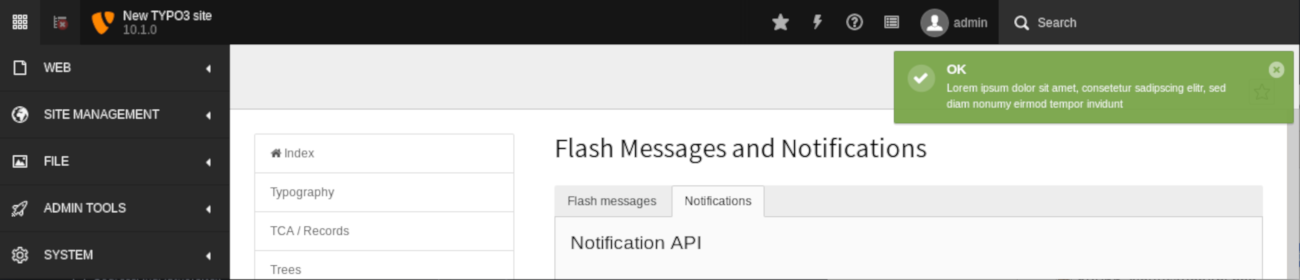
\includegraphics[width=0.90\linewidth]{ChangesForDevelopers/89066-NotificationApi.png}
%	\end{figure}
%
%\end{frame}

% ------------------------------------------------------------------------------
% Feature | 89061 | Introduce Notification Actions

\begin{frame}[fragile]
	\frametitle{Systeemwijzigingen}
	\framesubtitle{Berichtacties}

	\begin{itemize}
		\item JavaScript berichten in de backend ondersteunen nu actie(knoppen).
	\end{itemize}

	\begin{figure}
		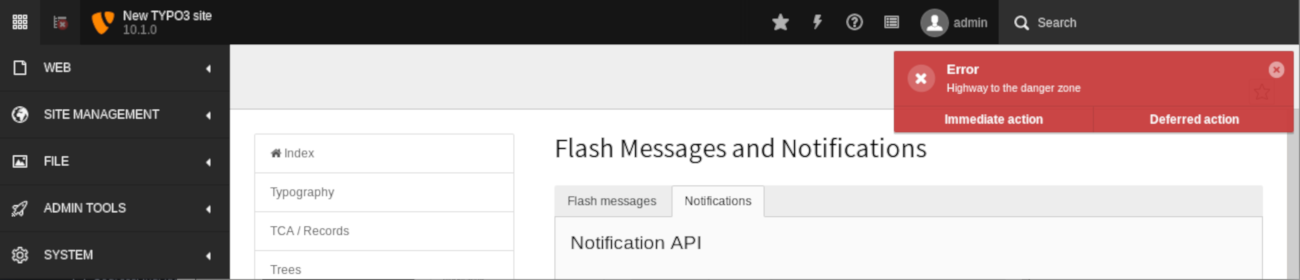
\includegraphics[width=0.90\linewidth]{InDepthChanges/89061-NotificationActionsAndButtons.png}
	\end{figure}

\end{frame}

% ------------------------------------------------------------------------------
% Feature | 89244 | Broadcast Channels and Messaging

\begin{frame}[fragile]
	\frametitle{Systeemwijzigingen}
	\framesubtitle{Uitzendkanalen en berichtgeving}

	% decrease font size for code listing
	\lstset{basicstyle=\tiny\ttfamily}

	\begin{itemize}
		\item Het is nu mogelijk om "uitzendberichten" met JavaScript te versturen en te ontvangen.
	\end{itemize}

	\vspace{-0.2cm}
	\begingroup
		\color{red}
			\begin{center}
				De API is voorlopig nog \textbf{intern}\newline
				en kan op elk moment wijzigen totdat het "stable" verklaard wordt.
			\end{center}
	\endgroup

	\begin{itemize}
		\item Voorbeeld voor het \textbf{versturen} van een bericht:
\begin{lstlisting}
require(['TYPO3/CMS/Backend/BroadcastService'], function (BroadcastService) {
  const payload = {
    componentName: 'my_extension',
    eventName: 'my_event',
    foo: 'bar'
  };
  BroadcastService.post(payload);
});
\end{lstlisting}

	\end{itemize}

\end{frame}

% ------------------------------------------------------------------------------
% Feature | 89244 | Broadcast Channels and Messaging

\begin{frame}[fragile]
	\frametitle{Systeemwijzigingen}
	\framesubtitle{Uitzendkanalen en berichtgeving}

	% decrease font size for code listing
	\lstset{basicstyle=\tiny\ttfamily}

	\begin{itemize}
		\item Voorbeeld voor het \textbf{ontvangen} van het bericht:
\begin{lstlisting}
define([], function() {
  document.addEventListener('typo3:my_component:my_event', (e) => eventHandler(e.detail));
  function eventHandler(detail) {
    // output contains key 'foo' as the payload
    console.log(detail);
  }
});
\end{lstlisting}

		\item Zie \href{https://developer.mozilla.org/en-US/docs/Web/API/Broadcast_Channel_API}{developer.mozilla.org} voor meer details.

	\end{itemize}

\end{frame}

% ------------------------------------------------------------------------------
% Feature | 88871 | Handle middleware handler in RequestFactory correctly

\begin{frame}[fragile]
	\frametitle{Systeemwijzigingen}
	\framesubtitle{RequestFactory Middleware Handler}

	% decrease font size for code listing
	\lstset{basicstyle=\tiny\ttfamily}

	\begin{itemize}
		\item Het is nu mogelijk om eigen middleware handlers als een array te definiëren.
		\item De RequestFactory bouwt een stapel handlers gebaseerd op de\newline
			\small
				\texttt{\$GLOBALS['TYPO3\_CONF\_VARS']['HTTP']['handler']}
			\normalsize
			array en injecteert het in de client.
		\item Bijvoorbeeld:
\begin{lstlisting}
use \TYPO3\CMS\Core\Utility\GeneralUtility;
use \Vendor\MyExtension\Middleware\Guzzle\CustomMiddleware;
use \Vendor\MyExtension\Middleware\Guzzle\SecondCustomMiddleware;

# Add custom middleware to default Guzzle handler stack
$GLOBALS['TYPO3_CONF_VARS']['HTTP']['handler'][] =
  (GeneralUtility::makeInstance(CustomMiddleware::class))->handler();
$GLOBALS['TYPO3_CONF_VARS']['HTTP']['handler'][] =
  (GeneralUtility::makeInstance(SecondCustomMiddleware::class))->handler();
\end{lstlisting}

	\end{itemize}

\end{frame}

% ------------------------------------------------------------------------------
% Feature | 88602 | Allow registering additional file processors

\begin{frame}[fragile]
	\frametitle{Systeemwijzigingen}
	\framesubtitle{Eigen Bestandsprocessors}

	% decrease font size for code listing
	\lstset{basicstyle=\tiny\ttfamily}

	\begin{itemize}
		\item Ontwikkelaars kunnen nu eigen bestandsprocessors registreren.
		\item Voeg de volgende code toe aan het bestand \texttt{ext\_localconf.php}:
\begin{lstlisting}
$GLOBALS['TYPO3_CONF_VARS']['SYS']['fal']['processors']['ExampleImageProcessor'] = [
  'className' => \Vendor\MyExtension\Resource\Processing\ExampleImageProcessor::class,
  'before' => 'LocalImageProcessor',
];
\end{lstlisting}

		\item Voorbeeld van gebruik:

			\begin{itemize}
				\item een watermerk toevoegen aan afbeeldingen
				\item geüploade bestanden comprimeren in een ZIP-bestand
				\item bewerkte kopieën van afbeeldingen opslaan
				\item etc.
			\end{itemize}

	\end{itemize}

\end{frame}

% ------------------------------------------------------------------------------
% Feature | 88950 | Add storeSession argument to Widget ViewHelpers

\begin{frame}[fragile]
	\frametitle{Systeemwijzigingen}
	\framesubtitle{Widget ViewHelpers}

	% decrease font size for code listing
	\lstset{basicstyle=\smaller\ttfamily}

	\begin{itemize}
		\item Widget ViewHelpers plaatsen in sommige situaties een sessie-cookie in de frontend.
		\item Omdat dit niet altijd gewenst is (bijv. de AVG), kan dit nu worden be\"{\i}nvloed.
		\item Een instelling \texttt{storeSession} is ge\"{\i}ntroduceerd voor ontwikkelaars om deze functie te kunnen in- of uitschakelen.
\begin{lstlisting}
<f:widget.autocomplete
  for="name"
  objects="{posts}"
  searchProperty="author"
  storeSession="false" />
\end{lstlisting}

	\end{itemize}

\end{frame}

% ------------------------------------------------------------------------------
% Feature | 89577 | New PSR-14 based events for File Abstraction Layer
% Deprecation | 89577 | FAL SignalSlot handling migrated to PSR-14 events

\begin{frame}[fragile]
	\frametitle{Systeemwijzigingen}
	\framesubtitle{PSR-14 Events in FAL}

	% decrease font size for code listing
	\lstset{basicstyle=\tiny\ttfamily}

	\begin{itemize}
		\item Ongeveer 40 nieuwe op
			\href{https://www.php-fig.org/psr/psr-14/}{PSR-14}
			gebaseerde Events zijn toegevoegd aan de bestandsabstractielaag (FAL).
		\item Ze vervangen bestaande Extbase Signal/Slots.
		\item De Signals kunnen gebruikt blijven (zonder een melding dat het verouderd is!).
			De Signals in FAL worden waarschijnlijk verwijderd in TYPO3 v11.
		\item Extensiebouwers wordt geadviseerd de code te migreren en Events te gebruiken.
		\item Bekijk de nieuwe PHP klassen om meer te leren over PSR-14.
	\end{itemize}

\end{frame}


% ------------------------------------------------------------------------------
% Deprecation | 89733 | Signal Slots in Core Extension migrated to PSR-14 events

\begin{frame}[fragile]
	\frametitle{Systeemwijzigingen}
	\framesubtitle{PSR-14 Events in de TYPO3 Core}

	\begin{itemize}
		\item Een aantal nieuwe PSR-14 Events vervangen Signal/Slots in de TYPO3 core:
			\newline

			\begin{itemize}\tiny
				\item \texttt{TYPO3\textbackslash
					CMS\textbackslash
					Core\textbackslash
					Imaging\textbackslash
					Event\textbackslash
					ModifyIconForResourcePropertiesEvent}
					\newline
				\item \texttt{TYPO3\textbackslash
					CMS\textbackslash
					Core\textbackslash
					DataHandling\textbackslash
					Event\textbackslash
					IsTableExcludedFromReferenceIndexEvent}
					\newline
				\item \texttt{TYPO3\textbackslash
					CMS\textbackslash
					Core\textbackslash
					DataHandling\textbackslash
					Event\textbackslash
					AppendLinkHandlerElementsEvent}
					\newline
				\item \texttt{TYPO3\textbackslash
					CMS\textbackslash
					Core\textbackslash
					Configuration\textbackslash
					Event\textbackslash
					AfterTcaCompilationEvent}
					\newline
				\item \texttt{TYPO3\textbackslash
					CMS\textbackslash
					Core\textbackslash
					Database\textbackslash
					Event\textbackslash
					AlterTableDefinitionStatementsEvent}
					\newline
				\item \texttt{TYPO3\textbackslash
					CMS\textbackslash
					Core\textbackslash
					Tree\textbackslash
					Event\textbackslash
					ModifyTreeDataEvent}
					\newline
				\item \texttt{TYPO3\textbackslash
					CMS\textbackslash
					Backend\textbackslash
					Backend\textbackslash
					Event\textbackslash
					SystemInformationToolbarCollectorEvent}
					\newline
			\end{itemize}

	\end{itemize}

\end{frame}

% ------------------------------------------------------------------------------
% Deprecation | 89718 | Legacy PageTSconfig parsing lowlevel API

\begin{frame}[fragile]
	\frametitle{Systeemwijzigingen}
	\framesubtitle{TSconfig Parsing}

	% decrease font size for code listing
	\lstset{basicstyle=\tiny\ttfamily}

	\begin{itemize}
		\item Twee nieuwe PHP-klassen zijn toegevoegd om Page TSconfig te laden en te parsen:
			\begin{itemize}\smaller
				\item \texttt{TYPO3\textbackslash
					CMS\textbackslash
					Core\textbackslash
					Configuration\textbackslash
					Loader\textbackslash
					PageTsConfigLoader}
				\item \texttt{TYPO3\textbackslash
					CMS\textbackslash
					Core\textbackslash
					Configuration\textbackslash
					Parser\textbackslash
					PageTsConfigParser}
			\end{itemize}

		\item For example:
\begin{lstlisting}
// Fetch all available PageTS of a page/rootline:
$loader = GeneralUtility::makeInstance(PageTsConfigLoader::class);
$tsConfigString = $loader->load($rootLine);

// Parse the string and apply conditions:
$parser = GeneralUtility::makeInstance(
  PageTsConfigParser::class, $typoScriptParser, $hashCache
);

$pagesTSconfig = $parser->parse($tsConfigString, $conditionMatcher);
\end{lstlisting}

	\end{itemize}

\end{frame}

% ------------------------------------------------------------------------------
% Important | 87518 | Use prepared statements for pdo_mysql per default

\begin{frame}[fragile]
	\frametitle{Systeemwijzigingen}
	\framesubtitle{Prepared Statements}

	% decrease font size for code listing
	\lstset{basicstyle=\tiny\ttfamily}

	\begin{itemize}
		\item Het \texttt{pdo\_mysql} stuurprogramma gebruikt nu standaard prepared statements.
		\item In TYPO3 < v10.2, worden \textit{nagebootste prepared statements} gebruikt.
			Dit betekent dat alle teruggegeven waarden van een query teksten zijn.
		\item Dit gedrag is gewijzigd en prepared statements worden gebruikt
			die de eigenlijke gegevenstypes teruggeven.
		\item Voorbeeld: waardes van een veld dat gedefinieerd is als geheel getal worden in PHP
			teruggegeven als \texttt{int}.
		\item Deze functie kan uitgeschakeld worden met de optie
			\texttt{PDO::ATTR\_EMULATE\_PREPARES} in de database-connectie.

	\end{itemize}

\end{frame}

% ------------------------------------------------------------------------------
% Feature | 87380 | Introduce SiteLanguageAwareInterface to denote site language awareness

\begin{frame}[fragile]
	\frametitle{Systeemwijzigingen}
	\framesubtitle{Aanduiding ondersteuning voor taal van site}

	% decrease font size for code listing
	\lstset{basicstyle=\tiny\ttfamily}

% A SiteLanguageAwareInterface with the methods setSiteLanguage(Entity\SiteLanguage $siteLanguage) and getSiteLanguage() has been introduced.
% The interface can be used to denote a class as aware of the site language.

	\begin{itemize}
		\item Een \texttt{SiteLanguageAwareInterface} is toegevoegd..
		\item De interface kan gebruikt worden om aan te duiden dat een klasse de taal
			van een site ondersteunt.
		\item Routering-aspecten die rekening houden met de taal van een site
			gebruiken nu de \texttt{SiteLanguageAwareInterface} naast
			de \texttt{SiteLanguageAwareTrait}.
	\end{itemize}

\end{frame}

% ------------------------------------------------------------------------------
% Important | 89645 | Removed systemLog options

\begin{frame}[fragile]
	\frametitle{Systeemwijzigingen}
	\framesubtitle{API voor systeemlog}

	% decrease font size for code listing
	\lstset{basicstyle=\tiny\ttfamily}

	\begin{itemize}
		\item De volgende opties zijn verwijderd uit de standaardconfiguratie van TYPO3:

			\begin{itemize}\smaller
				\item \texttt{\$GLOBALS['TYPO3\_CONF\_VARS']['SYS']['systemLog']}
				\item \texttt{\$GLOBALS['TYPO3\_CONF\_VARS']['SYS']['systemLogLevel']}
			\end{itemize}\normalsize

		\item Makers van extensies wordt aangeraden gebruik te maken van de log-API en de systeemlog-opties te verwijderen.
	\end{itemize}

\end{frame}

% ------------------------------------------------------------------------------
% Feature | 89603 | Introduce native pagination for lists

\begin{frame}[fragile]
	\frametitle{Systeemwijzigingen}
	\framesubtitle{Ingebouwde paginering van lijsten}

	% decrease font size for code listing
	\lstset{basicstyle=\tiny\ttfamily}

	\begin{itemize}
		\item Ondersteuning voor paginering van lijsten zoals array's of QueryResults van Extbase is nu ingebouwd.
		\item De \texttt{PaginatorInterface} definieert een aantal basisfuncties.
		\item De \texttt{AbstractPaginator} klasse bevat de belangrijkste logica van paginering.
		\item Hiermee kunnen allerlei soorten paginering gebouwd worden.
\begin{lstlisting}
use TYPO3\CMS\Core\Pagination\ArrayPaginator;

$items = ['appel', 'banaan', 'aardbei', 'framboos', 'ananas'];
$currentPageNumber = 3;
$itemsPerPage = 2;

$paginator = new ArrayPaginator($itemsToBePaginated, $currentPageNumber, $itemsPerPage);
$paginator->getNumberOfPages(); // resultaat: 3
$paginator->getCurrentPageNumber(); // resultaat: 3
$paginator->getKeyOfFirstPaginatedItem(); // resultaat: 5
$paginator->getKeyOfLastPaginatedItem(); // resultaat: 5
\end{lstlisting}

	\end{itemize}

\end{frame}

% ------------------------------------------------------------------------------
% Deprecation | 89579 | ServiceChains require an array for excluded Service keys

\begin{frame}[fragile]
	\frametitle{Systeemwijzigingen}
	\framesubtitle{Service API}

	\begin{itemize}
		\item Parameter \texttt{\$excludeServiceKeys} wordt gebruikt voor het overslaan van bepaalde services
			als deze geschakeld zijn.
		\item De parameter is gewijzigd van kommagescheiden lijst naar array in TYPO3 v10.2.
		\item Deze wijziging treft de Service API in de volgende componenten:

			\begin{itemize}
				\item \texttt{GeneralUtility::makeInstanceService()}
				\item \texttt{ExtensionManagementUtility::findService()}
			\end{itemize}

		\item Het doorgeven van een kommagescheiden lijst werkt maar is aangemerkt als \textbf{verouderd}.

	\end{itemize}

\end{frame}

% ------------------------------------------------------------------------------
% Feature | 86614 | Add PSR-14 event to control hreflang tags to be rendered

\begin{frame}[fragile]
	\frametitle{Systeemwijzigingen}
	\framesubtitle{Wijzig \texttt{hreflang}-tag}

	% decrease font size for code listing
	\lstset{basicstyle=\smaller\ttfamily}

	\begin{itemize}
		\item De \texttt{hreflang} tags kunnen gewijzigd worden voordat ze uitgevoerd worden.
		\item Ontwikkelaars kunnen dit bereiken door het registreren van een event listener voor dit event:\newline
			\smaller
				\texttt{TYPO3\textbackslash
					CMS\textbackslash
					Frontend\textbackslash
					Event\textbackslash
					ModifyHrefLangTagsEvent}
			\normalsize
	\end{itemize}

\end{frame}

% ------------------------------------------------------------------------------
% Feature | 88818 | Introduce events to modify CKEditor configuration

\begin{frame}[fragile]
	\frametitle{Systeemwijzigingen}
	\framesubtitle{CKEditor configuratie wijzigen}

	% decrease font size for code listing
	\lstset{basicstyle=\tiny\ttfamily}

	\begin{itemize}
		\item Met de volgende PSR-14-gebaseerde events kan de CKEditorconfiguratie worden gewijzigd:
\begin{lstlisting}
TYPO3\CMS\RteCKEditor\Form\Element\Event\AfterGetExternalPluginsEvent
TYPO3\CMS\RteCKEditor\Form\Element\Event\BeforeGetExternalPluginsEvent
TYPO3\CMS\RteCKEditor\Form\Element\Event\AfterPrepareConfigurationForEditorEvent
TYPO3\CMS\RteCKEditor\Form\Element\Event\BeforePrepareConfigurationForEditorEvent
\end{lstlisting}

		\item De
			\href{https://docs.typo3.org/c/typo3/cms-core/master/en-us/Changelog/10.3/Feature-88818-IntroduceEventsToModifyCKEditorConfiguration.html}{lijst wijzigingen}
			bevat een voorbeeld.
	\end{itemize}

\end{frame}

% ------------------------------------------------------------------------------
% Feature | 89738 | API for AJAX Requests

\begin{frame}[fragile]
	\frametitle{Systeemwijzigingen}
	\framesubtitle{API voor AJAX Requests}

	% decrease font size for code listing
	\lstset{basicstyle=\tiny\ttfamily}

	\begin{itemize}
		\item De \textbf{Fetch API} is toegevoegd voor het maken van AJAX requests
			en om TYPO3 minder afhankelijk van jQuery te maken.
		\item De API biedt een generieke definitie van Request en Response objecten
			(en andere zaken omtrent een netwerkrequest)
		\item Ondersteund door alle moderne browsers, zie
			\href{https://developer.mozilla.org/en-US/docs/Web/API/Fetch_API}{compatibiliteitsoverzicht}.
		\item De TYPO3 core gebruikt de nieuwe API al in de Install Tool, FormEngine en
			contextmenu's.
		\item Zie de
			\href{https://docs.typo3.org/c/typo3/cms-core/master/en-us/Changelog/10.3/Feature-89738-ApiForAjaxRequests.html}{lijst wijzigingen}
			voor enkele voorbeelden voor het gebruik van de Fetch API.

	\end{itemize}

\end{frame}

% ------------------------------------------------------------------------------
% Feature | 89650 | Allow line breaks in TCA descriptions

\begin{frame}[fragile]
	\frametitle{Systeemwijzigingen}
	\framesubtitle{TCA veld Beschrijving}

	\begin{itemize}
		\item Het veld Beschrijving in de TCA kan regeleindes bevatten om lange teksten beter leesbaar te maken.
	\end{itemize}

\end{frame}

% ------------------------------------------------------------------------------
% Important | 90020 | Legacy BasicFileUtility and ExtendedFileUtility classes marked as internal

\begin{frame}[fragile]
	\frametitle{Systeemwijzigingen}
	\framesubtitle{Klassen \texttt{BasicFileUtility} en \texttt{ExtendedFileUtility}}

	\begin{itemize}
		\item De volgende twee oude klassen zijn aangemerkt als \textbf{internal}
			en zouden niet meer gebruikt moeten worden:

			\begin{itemize}\small
				\item \texttt{TYPO3\textbackslash
					CMS\textbackslash
					Core\textbackslash
					Utility\textbackslash
					File\textbackslash
					BasicFileUtility}
				\item \texttt{TYPO3\textbackslash
					CMS\textbackslash
					Core\textbackslash
					Utility\textbackslash
					File\textbackslash
					ExtendedFileUtility}
			\end{itemize}

		\item Ontwikkelaars van extensies zouden de klasse \texttt{ResourceStorage}
			en \texttt{ResourceFactory} moeten gebruiken voor het beheer van assets.

	\end{itemize}

\end{frame}

% ------------------------------------------------------------------------------
% Feature | 89139 | Add dependency injection support for console commands

\begin{frame}[fragile]
	\frametitle{Systeemwijzigingen}
	\framesubtitle{Console commando's: Symfony DI Ondersteuning}

	\begin{itemize}
		\item Afhankelijkheden kunnen nu geïnjecteerd worden via constructor of andere injectietechnieken.
		\item Voeg de \texttt{console.command} tag toe aan commando klassen.
		\item Gebruik het tag-attribuut \texttt{command} om de commandonaam te specificeren.
		\item De optionele tagattribuut \texttt{schedulable} kan ingesteld worden op \texttt{false}
			om het commando uit de Taakplanner te houden.

		\item Zie
			\href{https://docs.typo3.org/c/typo3/cms-core/master/en-us/Changelog/10.3/Feature-89139-AddDependencyInjectionSupportForConsoleCommands.html}{lijst wijzigingen}
			voor een voorbeeld.
	\end{itemize}

\end{frame}

% ------------------------------------------------------------------------------
% Feature | 90168 | Introduce Modal Actions

\begin{frame}[fragile]
	\frametitle{Systeemwijzigingen}
	\framesubtitle{Actieknoppen in popups}

	% decrease font size for code listing
	\lstset{basicstyle=\tiny\ttfamily}

	\begin{itemize}
		\item Modal popups ondersteunen actieknoppen.
		\item Als een alternatief voor de bestaande \texttt{trigger}-optie kan de nieuwe
			optie \texttt{action} worden gebruikt.
		\item Bijvoorbeeld:
\begin{lstlisting}
Modal.confirm('Header', 'Some content', Severity.error, [
  {
	text: 'Gebaseerd op trigger()',
    trigger: function () {
      console.log('Vintage!');
    }
  },
  {
	text: 'Gebaseerd op action()',
    action: new DeferredAction(() => {
      return new AjaxRequest('/any/endpoint').post({});
    })
  }
]);
\end{lstlisting}

	\end{itemize}

\end{frame}

% ------------------------------------------------------------------------------
% Feature | 90471 | JavaScript Event API

\begin{frame}[fragile]
	\frametitle{Systeemwijzigingen}
	\framesubtitle{JavaScript Event API}

	\begin{itemize}
		\item Een nieuwe Event API geeft JavaScript ontwikkelaars een stabiel koppelvlak voor event listeners.
		\item De API handelt bekende valkuilen af zoals event delegation en event unbinding.
		\item Elke \textit{event strategy} biedt twee manieren om het te koppelen aan een listener
		\item De Event API biedt verschillende stategieën om even listeners af te handelen.
		\item Zie
			\href{https://docs.typo3.org/c/typo3/cms-core/master/en-us/Changelog/10.3/Feature-90471-JavaScriptEventAPI.html}{lijst wijzigingen}
			voor voorbeelden en verdere details.
	\end{itemize}

\end{frame}

% ------------------------------------------------------------------------------
% Feature | 88648 | Define Twitter Card Type In Page Properties
% Important | 86577 | Query parameters are now included in canonicalized URLs

\begin{frame}[fragile]
	\frametitle{Systeemwijzigingen}
	\framesubtitle{Diversen}

	% decrease font size for code listing
	\lstset{basicstyle=\tiny\ttfamily}

	\begin{itemize}

		\item Het type Twitter Card kan nu gekozen/geconfigureerd worden.
			Deze optie zorgt voor de metatag \texttt{twitter:card} in de frontend.
\begin{lstlisting}
page {
  meta {
    twitter:card = summary_large_image
    twitter:card.replace = 1
  }
}
\end{lstlisting}

		\item Alleen parameters die nodig zijn om de cHash te berekenen worden standaard meegenomen in genormaliseerde URL's.
			Extra parameters kunnen nu geconfigureerd worden:
\begin{lstlisting}
$GLOBALS['TYPO3_CONF_VARS']['FE']['additionalCanonicalizedUrlParameters'].
\end{lstlisting}

		\smaller
			Let op: voeg alleen parameters toe die de inhoud van de pagina wijzigen. Anders zien zoekmachines het wellicht als dubbele inhoud.
		\normalsize

	\end{itemize}

\end{frame}

% ------------------------------------------------------------------------------
% Breaking | 88681 | Import Of PHP Files In Import Export Files Removed
% Breaking | 88500 | RTE image handling functionality dropped
% Breaking | 81950 | Remove leftover workspaces unpublishing functionality

\begin{frame}[fragile]
	\frametitle{Systeemwijzigingen}
	\framesubtitle{Diversen}

	% decrease font size for code listing
	\lstset{basicstyle=\tiny\ttfamily}

	\begin{itemize}

		\item Bij het importeren van XML-data met \texttt{EXT:impexp} wordt het Patroon voor het weigeren van bestanden gebruikt en
			weigert nu bijvoorbeeld PHP bestanden.

		\item Ondersteuning voor afbeeldingen in de RTE is compleet verwijderd.
			Voor ondersteuning van afbeeldingen in CKEditor kan bijv. \texttt{EXT:rte\_ckeditor\_image} gebruikt worden.

		\item Een eigenschap binnen werkruimtes voor het \textit{de-publiceren} van records is verwijderd in v10
			(inclusief databaseveld \texttt{sys\_workspace.unpublish\_time}). Deze functie was uitgeschakeld
			in TYPO3 v4.5 en niet meer gebruikt of beschikbaar gesteld door TYPO3.

	\end{itemize}

\end{frame}

% ------------------------------------------------------------------------------
% Breaking | 88772 | JavaScript script tags omit type=text/javascript in HTML5
% Remove system extension EXT:rsaauth
% Remove system extension EXT:fe_edit

\begin{frame}[fragile]
	\frametitle{Systeemwijzigingen}
	\framesubtitle{Diversen}

	% decrease font size for code listing
	\lstset{basicstyle=\tiny\ttfamily}

	\begin{itemize}

		\item Bij het maken van HTML5 output krijgen \texttt{<script>} tags geen
			\texttt{type="text/javascript"} attribuut meer.

		\item Dit kan in TypoScript weer ingeschakeld worden indien nodig:
\begin{lstlisting}
page {
  includeJS {
    myfile = EXT:example/Resources/Public/JavaScript/myfile.js
    myfile.type = text/javascript
  }
}
\end{lstlisting}

		\item De volgende verouderde systeemextensies zijn verwijderd:

			\begin{itemize}
				\item \texttt{EXT:rsaauth}
				\item \texttt{EXT:fe\_edit}
			\end{itemize}

	\end{itemize}

\end{frame}

% ------------------------------------------------------------------------------
% Breaking | 88525 | Remove “createDirs” directive of extension installation / ext_emconf.php
% Breaking | 87511 | Remove $viewFormatToObjectNameMap property
% Breaking | 87511 | Remove $namespacesViewObjectNamePattern property
% Feature | 87726 | Extend Frontend Login Controller Hook To Validate Password

\begin{frame}[fragile]
	\frametitle{Systeemwijzigingen}
	\framesubtitle{Diversen}

	\begin{itemize}
		\item Optie \texttt{createDirs} in bestand \texttt{ext\_emconf.php} wordt niet meer ondersteund.

			\begin{itemize}\smaller
				\item[\ding{228}] Mappen worden niet meer automatisch aangemaakt tijdens installatie van de extensie.
			\end{itemize}\normalsize

		\item De volgende twee eigenschappen in klasse
			\texttt{TYPO3\textbackslash
				CMS\textbackslash
				Extbase\textbackslash
				Mvc\textbackslash
				Controller\textbackslash
				ActionController}\newline
			zijn verwijderd:

			\begin{itemize}
				\item \texttt{\$namespacesViewObjectNamePattern}
				\item \texttt{\$viewFormatToObjectNameMap}
			\end{itemize}

		\item De volgende bestaande hook is uitgebreid en kan nu
			ook gebruikt worden om wachtwoorden te valideren:\newline
			{\fontsize{8}{10} \selectfont \texttt{\$GLOBALS['TYPO3\_CONF\_VARS']['EXTCONF']['felogin']['password\_changed']}}

	\end{itemize}

\end{frame}

% ------------------------------------------------------------------------------
% Deprecation | 87613 | Deprecate /TYPO3/CMS/Extbase/Utility/TypeHandlingUtility::hex2bin
% Deprecation | 88554 | Deprecated methods in VersionNumberUtility

\begin{frame}[fragile]
	\frametitle{Systeemwijzigingen}
	\framesubtitle{Diversen}

	\begin{itemize}

		\item De volgende functies van klasse
			\smaller\texttt{\textbackslash
				TYPO3\textbackslash
				CMS\textbackslash
				Core\textbackslash
				Utility\textbackslash
				VersionNumberUtility}\normalsize\newline
			zijn als verouderderd aangemerkt:

			\begin{itemize}
				\item \texttt{convertIntegerToVersionNumber()}
				\item \texttt{splitVersionRange()}
				\item \texttt{raiseVersionNumber()}
			\end{itemize}

			\begin{itemize}\smaller
				\item[\ding{228}] Maak eigen functies hiervoor.
			\end{itemize}\normalsize

	\end{itemize}

\end{frame}

% ------------------------------------------------------------------------------
% Feature | 86964 | Allow getting class property default value
% Deprecation | 82669 | Streamline Backend route path inconsistencies

\begin{frame}[fragile]
	\frametitle{Systeemwijzigingen}
	\framesubtitle{Diversen}

	% decrease font size for code listing
	\lstset{basicstyle=\tiny\ttfamily}

	\begin{itemize}
		\item Het is nu mogelijk om de standaard waarde van een klasse-eigenschap
			te krijgen bij gebruik van de ReflectionService.
\begin{lstlisting}
$property = GeneralUtility::makeInstance(ReflectionService::class)
  ->getClassSchema(MyClass::class)
  ->getProperty('myProperty');
\end{lstlisting}

		\item Backend routes naar modules zonder pad-configuratie heten nu\newline
			standaard "\texttt{/module/<main-module>/<sub-module>}"\newline
			\small
				(voorbeeld: "\texttt{/module/web/ts}".)
			\normalsize

		\item Oude routes werken nog steeds (bijv. "\texttt{/web/ts/}") maar deze syntax zal verdwijnen in TYPO3 v11.

	\end{itemize}

\end{frame}

% ------------------------------------------------------------------------------
% Breaking | 88669 | FormEngine FormDataProvider parentPageTca removed
% Breaking | 88744 | Database fields related to CSS Styled Content removed
% Breaking | 88143 | Version-related database field “t3ver_id” removed
% Deprecation | 88746 | PageRepository PHP class moved from Frontend to Core Extension

\begin{frame}[fragile]
	\frametitle{Systeemwijzigingen}
	\framesubtitle{Diversen}

	\begin{itemize}
		\item De FormEngine DataProvider \texttt{parentPageTca} is verwijderd.

			\begin{itemize}\smaller
				\item[\ding{228}] Ontwikkelaars kunnen \texttt{\$GLOBALS['TCA']['pages']} direct gebruiken in plaats van \texttt{\$result['parentPageTca']}.
			\end{itemize}\normalsize

		\item De volgende database-velden zijn verwijderd:

			\begin{itemize}\smaller
				\item \texttt{tt\_content.spaceBefore} (vervangen door \texttt{space\_before\_class})
				\item \texttt{tt\_content.spaceAfter} (vervangen door \texttt{space\_after\_class})
				\item \texttt{pages.t3ver\_id} (ongebruikt sinds TYPO3 v9)
			\end{itemize}\normalsize

			\item De PHP klasse
				\texttt{\textbackslash
					TYPO3\textbackslash
					CMS\textbackslash
					Frontend\textbackslash
					Page\textbackslash
					PageRepository} is verplaatst van de "frontend" systeemextensie naar de core.

				\begin{itemize}\smaller
					\item Vervang door klasse:
						\texttt{\textbackslash
							TYPO3\textbackslash
							CMS\textbackslash
							Core\textbackslash
							Domain\textbackslash
							Repository\textbackslash
							PageRepository}
				\end{itemize}\normalsize

	\end{itemize}

\end{frame}

% ------------------------------------------------------------------------------
% Breaking | 88574 | 4th parameter of PageRepository>enableFields removed
% Deprecation | 85895 | Deprecate File::_getMetaData()
% Deprecation | 88662 | Deprecated backend route xMOD_tximpexp

\begin{frame}[fragile]
	\frametitle{Systeemwijzigingen}
	\framesubtitle{Diversen}

	\begin{itemize}

		\item 4e parameter van functie \texttt{PageRepository->enableFields()} is verwijderd.

			\begin{itemize}\smaller
				\item[\ding{228}] Als 4e parameter gebruikt wordt met de waarde "\textbf{false}" kan dit veilig verwijderd worden.
				\item[\ding{228}] Als het gebruikt wordt met waarde "\textbf{true}" dan moet de code vervangen worden met een aparte instantie van \texttt{PageRepository} met een eigen \texttt{Context}.
			\end{itemize}\normalsize

		\item De interne functie \texttt{File::\_getMetaData()}, gebruikt voor het ophalen van metadata van een bestand,
			is als verouderd aangemerkt.

			\begin{itemize}\smaller
				\item[\ding{228}] Gebruik \texttt{\$fileObject->getMetaData()->get()} om nu de metadata op te halen.
			\end{itemize}\normalsize

		\item De route identifier "\texttt{xMOD\_tximpexp}" is als verouderd aangemerkt.

			\begin{itemize}\smaller
				\item[\ding{228}] Gebruik \texttt{tx\_impexp\_export} of \texttt{tx\_impexp\_import} afhankelijk van de situatie.
			\end{itemize}\normalsize

	\end{itemize}

\end{frame}

% ------------------------------------------------------------------------------
% Breaking | 88496 | Method getSwitchableControllerActions has been removed
% Breaking | 87567 | Global variable $TBE_TEMPLATE removed
% Breaking | 88660 | $GLOBALS[T3_VAR] removed

\begin{frame}[fragile]
	\frametitle{Systeemwijzigingen}
	\framesubtitle{Diversen}

	\begin{itemize}

		\item De volgende abstracte functie is verwijderd:\newline
			\smaller
				\texttt{\textbackslash
					TYPO3\textbackslash
					CMS\textbackslash
					Extbase\textbackslash
					Configuration\textbackslash
					AbstractConfigurationManager::}\newline
					\texttt{getSwitchableControllerActions()}
			\normalsize

			\begin{itemize}\smaller
				\item[\ding{228}] Gebruik de nieuwe functienaam \texttt{getControllerConfiguration()} (zelfde PHP klasse).
			\end{itemize}\normalsize

		\item De globale variabele \texttt{\$TBE\_TEMPLATE} is verwijderd, inclusief
			de gerelateerde PSR-15 middeleware (die als intern was aangemerkt).

			\begin{itemize}\smaller
				\item[\ding{228}] Instantieer de DocumentTemplate klasse direct in de controller van de module.
				\item[\ding{228}] Migreer naar ModuleTemplate die sinds TYPO3 v7 beschikbaar is.
			\end{itemize}\normalsize

		\item De globale variabele \texttt{\$GLOBALS['T3\_VAR']} is verwijderd.\newline

	\end{itemize}

\end{frame}

% ------------------------------------------------------------------------------
% Important | 89001 | TSFE->createHashBase
% Feature | 89150 | Add events before and after rollback of record history entries

\begin{frame}[fragile]
	\frametitle{Systeemwijzigingen}
	\framesubtitle{Diversen}

	\begin{itemize}
		\item De \texttt{hashParameters} voor het berekenen van de hashBase zijn in de volgende klasse gewijzigde:\newline
			\small
				\texttt{TYPO3\textbackslash
					CMS\textbackslash
					Frontend\textbackslash
					Controller\textbackslash
					TypoScriptFrontendController}
			\normalsize

			\begin{itemize}
				\item \texttt{gr\_list} is vervangen door \texttt{groupIds}.
				\item \texttt{cHash} is vervangen door \texttt{dynamicArguments}.
				\item \texttt{domainStartPage} is vervangen door \texttt{site} (site identifier).
			\end{itemize}

		\item Twee nieuwe gebeurtenissen worden verstuurd als records teruggedraaid worden:

			\begin{itemize}\smaller
				\item \texttt{TYPO3\textbackslash
					CMS\textbackslash
					Backend\textbackslash
					History\textbackslash
					Event\textbackslash
					BeforeHistoryRollbackStartEvent}
				\item \texttt{TYPO3\textbackslash
					CMS\textbackslash
					Backend\textbackslash
					History\textbackslash
					Event\textbackslash
					AfterHistoryRollbackFinishedEvent}
			\end{itemize}\normalsize

	\end{itemize}

\end{frame}

% ------------------------------------------------------------------------------
% Feature | 88805 | Add type to TYPO3/CMS/Core/Database/Query/QueryBuilder::set()

\begin{frame}[fragile]
	\frametitle{Systeemwijzigingen}
	\framesubtitle{Diversen}

	\begin{itemize}
		\item Methode \texttt{set()} van de querybouwer kent nu een 4e parameter
			om het type van de parameter met naam te specificeren:\newline
			\small
				\texttt{TYPO3\textbackslash
					CMS\textbackslash
					Core\textbackslash
					Database\textbackslash
					Query\textbackslash
					QueryBuilder::set()}
			\normalsize\newline
			\vspace{0.2cm}
			(de standaard is \texttt{\textbackslash PDO::PARAM\_STR})

	\end{itemize}

\end{frame}

% ------------------------------------------------------------------------------
% Feature | 21638 | Introduced IP locking for IPv6
% Breaking | 21638 | AbstractUserAuthentication::lockIP property removed

\begin{frame}[fragile]
	\frametitle{Systeemwijzigingen}
	\framesubtitle{Diversen}

	% decrease font size for code listing
	\lstset{basicstyle=\tiny\ttfamily}

	\begin{itemize}

		\item De functie voor het vastzetten op IP is uitgebreid om ook IPv6 te ondersteunen
			(frontend en backend).
\begin{lstlisting}
$GLOBALS['TYPO3_CONF_VARS']['FE']['lockIPv6'] = 2;
$GLOBALS['TYPO3_CONF_VARS']['BE']['lockIPv6'] = 2;
\end{lstlisting}

		\item De publieke eigenschap \texttt{lockIP} in de volgende PHP-klasse is verwijderd:\newline
			\small
				\texttt{\textbackslash
					TYPO3\textbackslash
					CMS\textbackslash
					Core\textbackslash
					Authentication\textbackslash
					AbstractUserAuthentication}.
			\normalsize

		\item Migratiemogelijkheden:

			\begin{itemize}\smaller
				\item[\ding{228}] Stel \texttt{lockIP} en \texttt{lockIPv6} in binnen \texttt{\$GLOBALS['TYPO3\_CONF\_VARS'][...]}.
				\item[\ding{228}] Gebruik de nieuwe IP-Locker API:
					\texttt{\textbackslash
						TYPO3\textbackslash
						CMS\textbackslash
						Core\textbackslash
						Authentication\textbackslash
						IpLocker}.
			\end{itemize}\normalsize

	\end{itemize}

\end{frame}

% ------------------------------------------------------------------------------
